\documentclass[journal,comsoc]{IEEEtran}
\usepackage[T1]{fontenc}
\usepackage[utf8]{inputenc}
\usepackage{amsmath,amssymb,amsfonts,amsthm}
\usepackage{mathrsfs}
\usepackage{enumitem}
\usepackage{graphicx}
\usepackage{textcomp}
\usepackage{xcolor}
\usepackage{booktabs}
\usepackage{url}
\usepackage[sort,compress]{cite}
\usepackage[ruled,vlined]{algorithm2e}
\usepackage[justification=centering,labelsep=period]{caption}
\captionsetup[table]{name=TABLE}
\renewcommand{\thetable}{\arabic{table}}

\newtheorem{theorem}{Theorem}
\newtheorem{lemma}{Lemma}
\newtheorem{proposition}{Proposition}

\interdisplaylinepenalty=2500

\begin{document}

\title{Distributed Quantum-Assisted Robust AoII Minimization in Satellite-Ground Integrated Edge Networks}
\author{Mohammad~Arif~Hossain,~\IEEEmembership{Member,~IEEE}, Tanzimul~Alam~Fahim,~Weiqi~Liu,~\IEEEmembership{Member,~IEEE}, and~Nirwan~Ansari,~\IEEEmembership{Life~Fellow,~IEEE}%
\thanks{Mohammad~Arif~Hossain is with Department of Engineering Technology and Quantum Research Interdisciplinary Science and Education (QRISE) Center at Middle Tennessee State University (MTSU), TN 37132 USA (e-mail: Mohammad.Hossain@mtsu.edu), Tanzimul~Alam~Fahim is with the Computational Science PhD Program at MTSU, Murfreesboro, TN 37132 USA, Weiqi Liu is with the Department of Computer Science and Computer Information Systems, Auburn University at Montgomery, AL 36117 USA, and Nirwan Ansari is with the Department of Electrical and Computer Engineering, New Jersey Institute of Technology, NJ 07102 USA.}}

\maketitle

% Abstract and Sections I to IV
\begin{abstract}
Edge servers that act on a monitored process need an estimate that is correct, not merely recent. In
satellite-ground integrated networks (SAGIN), satellite handover and shadowing interrupt links for long enough that the
monitored process can change state several times, so the age of incorrect information (AoII) is the appropriate
measure of estimation quality. This paper formulates the robust, network-level AoII minimization problem VANGUARD, in
which update rates, serving-node association, and bandwidth are chosen jointly to minimize the worst-case time-average
AoII over a set of disruption scenarios, and solves it with SENTINEL, a distributed hybrid quantum-classical procedure.
A renewal-interval decomposition turns the history-dependent AoII into a closed-form cost per inter-delivery
interval. The minimax over scenarios is dualized into scenario weights updated by a classical outer loop, so that each
satellite-ground domain solves a linear assignment subproblem encoded as a compact quadratic unconstrained binary
optimization (QUBO) whose one-hot structure is enforced by XY mixers rather than penalties; the domains are coordinated
through the sharing form of ADMM, and every returned schedule is certified by its exact worst-case AoII. The
evaluation uses Starlink ephemerides, the 3GPP TR 38.811 non-terrestrial channel, and acknowledgement feedback for
all policies, with an exact integer-programming reference and paired tests over 30 to 60 seeds. The
certificate held in 98.7\% of orchestration epochs under real passes; the robust schedule's certified worst case is 2
to 7\% below that of the nominal schedule at no measurable cost in realized AoII, and SENTINEL combined with a
state-aware transmission trigger comes within 10 to 20\% of the best per-slot heuristic while retaining the
certificate. Without failure feedback every policy degrades by an order of magnitude and the hybrid is 25 to 30\%
better than the per-slot heuristic at the larger network sizes. The quantum step is exact through 25 UEs in simulation with four to five times
fewer qubits than a direct epigraph encoding, and thirteen domains of 8 to 38 qubits sampled on two IBM Heron
processors all decoded to the exact optimum, with the fraction of usable shots falling from 86\% to 2.6\% over that
range. At these sizes the quantum sampler is correct but not a better optimizer than greedy association, and we report
this limit together with the scale at which it would matter.
\end{abstract}

\begin{IEEEkeywords}
6G, age of incorrect information (AoII), alternating direction method of multipliers (ADMM), mission-critical edge
computing, non-terrestrial networks, quantum approximate optimization algorithm (QAOA), remote estimation, robust
optimization, satellite-ground integrated network (SAGIN)
\end{IEEEkeywords}

\IEEEpeerreviewmaketitle

%=======================================================================
\section{Introduction}
%=======================================================================

Sixth-generation networks are expected to place decision-making at the edge~\cite{Saad2020}: an edge server that
monitors a hazard indicator, the integrity of a structure, or the position of an asset must act on its own estimate of
that process, often without a human in the loop. What matters to such a server is whether its estimate is still
correct. Terrestrial mobile edge computing provides capacity and low delay where ground infrastructure exists, which is
often not where monitoring is most needed, and satellite links extend coverage to the remaining regions at the price of
intermittent connectivity~\cite{Giordani2021}. The combination, a satellite-ground integrated network (SAGIN), is the
setting of this paper.

Satellite links fail in ways that terrestrial links rarely do. A low-earth-orbit satellite sets and hands the user over
to the next one every few minutes; buildings and foliage block the line of sight for the length of a pass; shadow
fading in the non-line-of-sight state exceeds ten decibels~\cite{TR38811}. During any of these interruptions the
monitored process keeps evolving, and by the time the link is restored the edge estimate may be wrong by several
states rather than simply old. The age of information (AoI)~\cite{Kaul2012, Yates2021} measures only elapsed time and
cannot tell these two situations apart. The age of incorrect information (AoII)~\cite{Maatouk2020, Maatouk2023} can:
it is zero while the estimate is correct and grows with the duration and the magnitude of a mismatch. AoII has been
analyzed mainly for one source and one monitor on a point-to-point channel. Carrying it to a network of edge nodes,
satellites, and base stations raises two difficulties. The metric depends on the whole trajectory of the source since
the estimate was last correct, so it does not fit the per-slot cost structure of the assignment problems used for
SAGIN resource allocation. And the duration of a mismatch is governed by outages whose length is uncertain, so the
allocation must be judged by its worst case over plausible disruptions, not by its average.

We treat the problem as robust combinatorial optimization. The first step is a renewal-interval decomposition: a source
that evolves as a Markov chain with known transition matrix accumulates, between two deliveries, an expected AoII that
depends only on the length of the interval, and this quantity can be tabulated offline. The channel then enters the
objective through a single number per scenario, the inter-delivery interval, and the resulting robust scheduling
problem, VANGUARD, is a minimax assignment problem over binary variables. The second step concerns how such a problem
can be given to a quantum solver. A direct encoding of the minimax, with an epigraph variable and one slack register
per scenario, needs three to four auxiliary qubits for every decision qubit and a penalty landscape in which classical
and quantum local search alike fail to find a feasible point; we document this failure in Section~VI. SENTINEL instead
dualizes the minimax into scenario weights that a classical outer loop updates by exponentiated gradient, so that each
inner subproblem has a linear objective and is encoded as a compact QUBO over the decision variables and a few
capacity-slack bits. The one-hot constraint of each user is enforced by the XY mixer of the quantum circuit rather
than by a penalty~\cite{Hadfield2019}, which keeps every sample a valid assignment. The network is partitioned into
satellite-ground domains that are coordinated by the sharing form of ADMM~\cite{Boyd2011}, and each assembled schedule
is evaluated exactly under every scenario, so the reported worst case is a certificate that does not rest on the
solver's optimality.

The third step is an evaluation that a reader can trust. Satellite passes are propagated from a Starlink
two-line-element snapshot with SGP4~\cite{Vallado2006}; the large-scale channel follows the suburban tables of
3GPP TR 38.811~\cite{TR38811}, including the elevation-dependent line-of-sight probability and clutter loss; every
policy, including the baselines, receives acknowledgement feedback and may abandon a link that has failed for a fixed
time; an integer linear program solved to optimality provides the reference for every solver; and all policies run on
the same random episodes, so that comparisons are paired and are reported with signed-rank tests. The quantum step is
run on two IBM Heron processors as well as in simulation.

The results support a modest and precisely stated set of claims. Under real passes the worst-case certificate held in
98.7\% of orchestration epochs, and its violations are non-line-of-sight passes whose clutter loss exceeds the
scenario set. The robust schedule's certificate is 2 to 7\% lower than that of its nominal counterpart in 67 to 100\%
of seeds, while the two are statistically indistinguishable in realized AoII, with and without failure feedback; the
value of the scenario set is the guarantee, not a lower average. A per-slot policy that transmits whenever its
observed AoII is positive is the strongest heuristic when feedback is available, and we show that it coincides with
the Whittle-index scheduler of the restless-bandit literature~\cite{Whittle1988, Kadota2018} at the bandwidths of this
study; SENTINEL combined with the same trigger comes within 10 to 20\% of it while keeping the certificate, and is 25 to
30\% better than it at 15 to 20 users when feedback is removed. The compact formulation is exact through 25 users and
within 12\% at 50 with four to five times fewer qubits than the epigraph encoding; its limit at 75 to 100 users is the
coordination of shared satellites, not the inner solver. On hardware, thirteen domains of 8 to 38 qubits sampled on
\texttt{ibm\_kingston} and \texttt{ibm\_fez} all decoded to the exact optimum, with the fraction of usable shots
decreasing from 86\% to 2.6\% as the circuits grew; a trained proximal-policy-optimization agent, included because
learning-based baselines are expected, matches the nominal schedule at five users and falls behind as its action
space grows. On every instance that fits a current device, greedy association is already optimal, so the quantum step
is a correct, hardware-runnable constrained sampler and not yet a better optimizer; the instances on which greedy
loses need one to two hundred qubits per domain.

The contributions of this paper are the following.
\begin{itemize}[leftmargin=13pt]
\item The robust scheduling problem VANGUARD, which minimizes the worst-case time-average AoII of a network of
monitored edge nodes over a scenario set of satellite shadowing and handover disruptions, jointly over update rates,
association, and bandwidth, subject to capacity, visibility, rate, and AoII-budget constraints.
\item A renewal-interval decomposition that expresses the expected AoII accumulated between deliveries in closed form
as a function of the interval length and the source's transition matrix, verified against Monte Carlo simulation to
within one percent, which reconciles the history dependence of AoII with binary-variable optimization.
\item SENTINEL, a distributed hybrid procedure in which the minimax is dualized into classically updated scenario
weights, each domain's subproblem is a compact QUBO with XY-mixer-enforced one-hot structure, candidate pruning
removes dominated combinations without changing the optimum, and the sharing form of ADMM with a warm start and a
cost-scaled penalty coordinates the domains; together with a certificate of the worst-case AoII of every schedule.
\item An evaluation under Starlink ephemerides and the TR 38.811 channel, against an exact integer-programming
reference, with paired statistics over 30 to 60 seeds, baselines that include the Whittle-index scheduler and a
trained learning agent, an ablation of failure feedback, sensitivity to the scenario set and to bandwidth, and runs of
the quantum step on two superconducting processors, with the scale limit of the quantum step stated explicitly.
\end{itemize}

The remainder of the paper is organized as follows. Section~II reviews related work. Section~III presents the system
model: the channel and satellite geometry, the monitored sources, the disruption scenarios, the renewal-interval
decomposition, the binary decision model, and the orchestration architecture. Section~IV formulates VANGUARD and its
binary reformulations. Section~V develops the dualized compact QUBO, the XY-mixer QAOA, and the ADMM coordination.
Section~VI reports the evaluation, and Section~VII concludes.

%=======================================================================
\section{State of the Art}
%=======================================================================

The paper touches five bodies of work: satellite-ground integrated edge computing, information freshness and
correctness, robust resource allocation, learning-based scheduling, and quantum-assisted combinatorial optimization.
We take them in turn and then state the gap.

\subsubsection{Satellite-Ground Integrated Edge Computing}
Mobile edge computing~\cite{Mao2017} has been extended beyond terrestrial coverage by placing edge servers on
satellites and base stations~\cite{Liu2018, Kato2019, Zhang2019}. The literature is dominated by task offloading
under deterministic or average channel assumptions~\cite{Cheng2019, Zhou2021}, with the completion delay of a task as
the objective. The correctness of what the server believes about the monitored process has not been the quantity
optimized. On the channel side, the 3GPP study on non-terrestrial networks~\cite{TR38811} provides
elevation-dependent line-of-sight probabilities, clutter losses, and shadow-fading statistics for several
environments, and the SGP4 propagator with public two-line elements~\cite{Vallado2006} gives pass geometry for any
constellation; most SAGIN evaluations use neither, and we found that the choice matters, because with real passes the
dominant disruptions are handovers and non-line-of-sight passes rather than coverage gaps.

\subsubsection{Age of Information and Age of Incorrect Information}
AoI has been studied extensively as a timeliness measure~\cite{Kaul2012, Kosta2017, Sun2017, Kadota2018, Yates2021}.
It is content-agnostic. AoII~\cite{Maatouk2020} penalizes the duration and magnitude of estimation error and has been
analyzed for a single source under threshold and semi-Markov policies~\cite{Maatouk2023, Kriouile2021} and over
unreliable, power-constrained channels~\cite{Chen2021}. For scheduling several sources over shared channels the
standard tool is the Whittle index of the restless bandit~\cite{Whittle1988}, applied to AoI by Kadota et
al.~\cite{Kadota2018}; it remains the reference policy against which new AoII schedulers should be measured, and we
include it. What is missing is a formulation in which association, bandwidth, and update rates are chosen jointly
across heterogeneous serving nodes, under outages that span several source transitions, with a guarantee on the
worst case.

\subsubsection{Robust Resource Allocation Under Link Uncertainty}
Robust optimization minimizes cost against the worst realization of an uncertain parameter in a bounded
set~\cite{BenTal2009, Bertsimas2004}. When the uncertainty set is a finite list of scenarios, the minimax can be
written as a maximization over scenario weights in the simplex, and the saddle point can be approached by
multiplicative-weights or exponentiated-gradient updates on the weights~\cite{Arora2012}; this is the mechanism we use
to keep the quantum subproblem linear. Robust allocation in satellite-ground edge computing has treated the
uncertainty as a perturbation of rate or delay, not as the driver of estimation error.

\subsubsection{Learning-Based Scheduling}
Deep reinforcement learning~\cite{Mnih2015, Schulman2017} has been applied to AoI- and AoII-aware scheduling in
point-to-point and small multi-user systems. It optimizes an expected return, needs training on representative
disruption patterns, and provides no bound on the estimation error under disruptions outside its training
distribution. These properties do not disqualify it as a baseline, and we train one with the same reward, feedback,
and episodes as every other policy; they do explain why a certified worst case is a different kind of guarantee.

\subsubsection{Quantum-Assisted Combinatorial Optimization}
QUBO formulations~\cite{Lucas2014, Glover2019} solved by the quantum approximate optimization algorithm
(QAOA)~\cite{Farhi2014, Cerezo2021} or by annealing~\cite{Albash2018} have been proposed for channel assignment and
scheduling in wireless networks~\cite{Kim2019}. Two developments bear directly on constrained assignment problems.
The alternating-operator form of QAOA~\cite{Hadfield2019} replaces the transverse-field mixer by one that preserves a
constraint subspace, so that one-hot and cardinality constraints need no penalty terms; and the concentration of
optimal QAOA parameters across instances~\cite{Brandao2018} allows angles optimized on a small instance to be reused
on a larger one that cannot be simulated. On present devices, error suppression by dynamical
decoupling~\cite{Viola1999} and randomized compiling~\cite{Wallman2016} is inexpensive, and we report its effect on our
circuits. QAOA has not previously been applied to a freshness or correctness objective, and reports of its use for
network resource allocation rarely state at what size the quantum sampler stops being competitive with a classical
heuristic on the same instances.

\subsubsection{Research Gap}
No existing work formulates AoII as a robust minimax multi-node scheduling problem with joint association and
resource allocation, targets information correctness rather than delay in robust SAGIN allocation, or applies
quantum-assisted optimization to a correctness objective with an encoding that a current device can execute.
SENTINEL addresses these three points, and its evaluation is designed so that the reader can see where each of its
components helps and where it does not.

%=======================================================================
\section{System Model}
%=======================================================================

\begin{figure}[!t]\centering
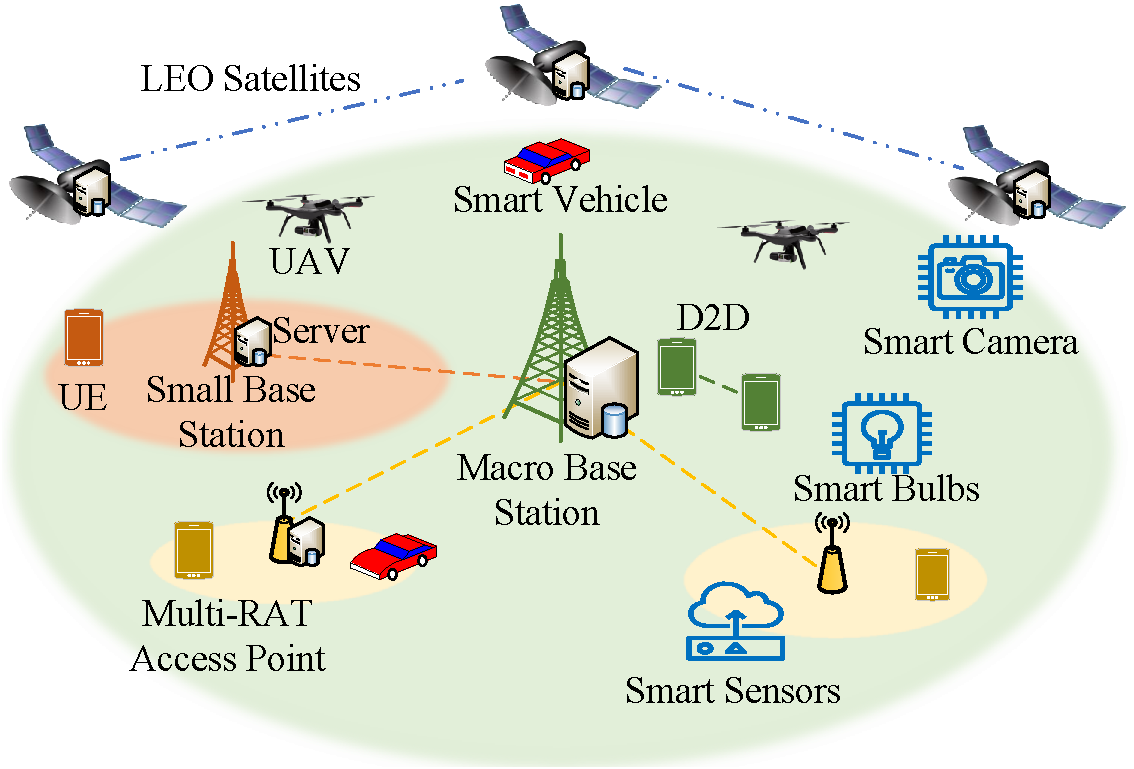
\includegraphics[width=0.9\columnwidth]{figures/SAGIN.pdf}
\caption{Correctness-aware monitoring over a satellite-ground integrated network under satellite disruption.}
\label{Fig1}
\end{figure}

We consider a satellite-ground integrated edge network in which monitoring edge nodes (UEs) observe time-varying
physical processes and transmit status updates to edge servers hosted at terrestrial base stations (BSs) or at
visible low-earth-orbit satellites (SATs). Let $\mathscr{U}$, $\mathscr{S}$, and $\mathscr{B}$ denote the sets of UEs,
SATs, and BSs, indexed by $u_i$, $s_j$, and $b_n$, and let $\mathscr{M}=\mathscr{S}\cup\mathscr{B}$ be the set of
serving nodes. Each serving node hosts an edge server that keeps a running estimate of every process assigned to it
and acts on that estimate. Time is slotted with slot duration $T_s$. UEs have low mobility over a decision interval;
the satellite topology changes continuously because of orbital motion. Table~\ref{tab:notation} lists the notation.

In contrast to the task-offloading models that dominate SAGIN edge computing, the quantity of interest here is the
correctness of the server's estimate. It depends on the dynamics of the monitored process, on when the UE samples and
transmits, and on whether the transmission is delivered before the process moves again. Satellite handover and
shadowing make the last of these uncertain, and an allocation chosen under nominal channel conditions can leave the
server with an estimate that is wrong rather than late.

The network is partitioned into $K$ local satellite-ground domains $\mathcal{D}_k=(\mathscr{U}_k,\mathscr{S}_k,
\mathscr{B}_k)$, $k\in\mathscr{K}=\{1,\ldots,K\}$, where the UE subsets partition $\mathscr{U}$ and a SAT may be
visible to several domains. Each domain has a classical controller that builds and solves a local robust binary
problem with a hybrid QAOA solver; a classical coordinator reconciles the bandwidth of SATs shared across domains and
certifies every assembled network schedule by its exact worst-case AoII.

\begin{table}[!t]
\centering
\caption{Key Notations}
\label{tab:notation}
\footnotesize
\renewcommand{\arraystretch}{1.15}
\begin{tabular}{|p{0.27\columnwidth}|p{0.61\columnwidth}|}
\hline
\textbf{Symbol} & \textbf{Definition} \\
\hline
$\mathscr{U}$, $\mathscr{S}$, $\mathscr{B}$ & Sets of UEs, SATs, and BSs \\
\hline
$\mathscr{M}=\mathscr{S}\cup\mathscr{B}$ & Set of serving nodes \\
\hline
$\mathscr{K}$, $\mathcal{D}_k$ & Set of domains; $k$-th domain \\
\hline
$\alpha_{ij}$, $\omega_{in}$ & Association of $u_i$ with $s_j$, $b_n$ \\
\hline
$\beta^{us}_{ij}$, $\beta^{ub}_{in}$ & Bandwidth allocated to $u_i$ by $s_j$, $b_n$ \\
\hline
$B^{s}_{j}$, $B^{b}_{n}$ & Bandwidth capacity of $s_j$, $b_n$ \\
\hline
$R^{us}_{ij}(\ell)$, $R^{ub}_{in}$ & Uplink rate of $u_i$ to $s_j$ (scenario $\ell$), to $b_n$ \\
\hline
$V_{ij}(t)$, $\Theta$ & Elevation of $s_j$ at $u_i$; minimum elevation \\
\hline
$G^{u}$, $G^{s}$, $G^{b}$ & Antenna gains of the UE, SAT, and BS \\
\hline
$\lambda^{\mathrm{cl}}$, $\sigma_{\mathrm{sf}}$ & TR 38.811 clutter loss; shadow-fading deviation \\
\hline
$\mathscr{L}$, $\Omega$ & Scenario set ($L$ scenarios); uncertainty set \\
\hline
$T^{\mathrm{dis}}(\ell)$, $\tau_{imq}(\ell)$ & Disruption window; induced outage (slots) \\
\hline
$T_s$, $D_i$ & Slot duration; status-update size (bits) \\
\hline
$X_i(t)$, $\hat{X}_i(t)$ & Monitored source of $u_i$; edge estimate \\
\hline
$\mathcal{X}_i$, $P_i$, $\pi_i$ & State space, transition matrix, stationary distribution \\
\hline
$f_i(x,\hat{x})$ & Distortion function \\
\hline
$\Delta_i^{II}(t)$, $\Delta_i^{II,\max}$ & Instantaneous AoII; AoII budget \\
\hline
$t_{i,\kappa}$, $Y_{i,\kappa}$ & $\kappa$-th delivery slot; inter-delivery interval \\
\hline
$\Psi_i(Y)$ & Expected AoII accumulated over an interval of length $Y$ \\
\hline
$\rho_i$, $\bar\rho_i^{h}$ & Update rate of $u_i$; $h$-th rate level ($H_i$ levels) \\
\hline
$\bar\beta_m^{q}$ & $q$-th bandwidth level of node $m$ ($Q_m$ levels) \\
\hline
$x_{imqh}$ & $1$ if $u_i$ uses node $m$, bandwidth level $q$, rate level $h$ \\
\hline
$\mathscr{A}_i$, $\mathscr{C}_i$ & Admissible combinations of $u_i$; pruned candidates \\
\hline
$\psi^{(\ell)}_{imqh}$ & Time-average AoII cost under scenario $\ell$ \\
\hline
$\mathbf{w}$, $\eta$ & Scenario weights; worst-case AoII (epigraph) \\
\hline
$T^{\mathrm{f}}$, $T^{\mathrm{b}}$ & Failure-detection window; blocking duration (slots) \\
\hline
$z_{jk}$, $u_{jk}$, $\varrho$ & ADMM bandwidth target, scaled dual, penalty \\
\hline
\end{tabular}
\end{table}

\subsection{Satellite Geometry and Communications Model}

Satellite positions are obtained from a constellation ephemeris. In the evaluation we propagate a public two-line
element set with SGP4~\cite{Vallado2006}, but the model only requires, for every SAT $s_j$ and UE $u_i$, the slant
range $d^{us}_{ij}(t)$ and the elevation angle $V_{ij}(t)$ in each slot. A SAT can serve $u_i$ in slot $t$ only if
$V_{ij}(t)\geq\Theta$. Each UE is served by the SAT that it has been handed to and keeps that SAT until it sets below
$\Theta$, at which point the UE is handed over to the SAT with the highest elevation; a dense constellation therefore
produces a sequence of passes of several minutes each, separated by handover interruptions, and no coverage gaps at
the elevation masks considered here.

The nominal path loss (in dB) between $u_i$ and $s_j$ is
\begin{equation}
    \varphi^{us}_{ij}=\varsigma^{us}+\zeta^{us}\log_{10}\!\left(f_{c}^{us}\right)
    +\xi^{us}\log_{10}\!\left(d^{us}_{ij}\right)+\lambda^{\mathrm{atm}}(V_{ij}),
\end{equation}
where $f_c^{us}$ is the carrier frequency, $\varsigma^{us}$, $\zeta^{us}$, and $\xi^{us}$ are the reference loss and
the frequency and distance exponents of free-space propagation, and $\lambda^{\mathrm{atm}}(V)$ is the atmospheric
absorption, which scales with $1/\sin V$. The UE-BS path loss $\varphi^{ub}_{in}$ uses the ground distance $d^{ub}_{in}$
and a terrestrial exponent $\xi^{ub}>2$ with a fixed margin. The received power at the SAT is
$p_i+G^{u}+G^{s}-\varphi^{us}_{ij}$ in dBm, where $p_i$ is the UE transmit power and $G^{u}$ and $G^{s}$ are the
antenna gains of the UE terminal and the satellite; the BS link uses $G^{b}$ in place of $G^{s}$ and the UE's sub-6-GHz
gain. The nominal uplink rate from $u_i$ to $s_j$ with bandwidth $\beta^{us}_{ij}$ is
\begin{equation}
    R^{us}_{ij}=\beta_{ij}^{us}\,\min\!\left\{\log_{2}\!\left(1+
    \frac{10^{(p_{i}+G^{u}+G^{s}-\varphi^{us}_{ij})/10}}{N_0\,\beta^{us}_{ij}\,F^{s}}\right),\ \bar{\gamma}\right\},
    \label{eq:rate_us}
\end{equation}
where $N_0$ is the noise power spectral density, $F^{s}$ the receiver noise figure, and $\bar\gamma$ the spectral
efficiency of the highest modulation and coding scheme. The UE-BS rate $R^{ub}_{in}$ is defined in the same way. Each
serving node divides its bandwidth among the UEs it serves, so the rate of a link does not depend on the association
decisions of other UEs once the bandwidth level is fixed. We treat co-channel interference as absorbed in the noise
figure and do not model residual Doppler, which the NTN frequency pre-compensation removes to within the subcarrier
spacing.

\emph{Large-scale channel.} On top of the nominal loss, each satellite link carries a large-scale state drawn once per
pass from the TR 38.811 model~\cite{TR38811}: with the elevation-dependent probability $p_{\mathrm{LOS}}(V)$ of the
chosen environment the pass is in line of sight; otherwise it is in non-line-of-sight and carries the clutter loss
$\lambda^{\mathrm{cl}}(V)$ of the carrier band, which at Ku band and suburban elevations is 17 to 25 dB. A shadow-fading
term with the state-dependent standard deviation $\sigma_{\mathrm{sf}}(V)$ is drawn per pass, and a small-scale fading
term per slot. In the suburban environment used in Section~VI roughly one pass segment in twenty is in
non-line-of-sight, and such a pass blocks the link for its whole duration at any bandwidth level.

\subsection{Monitored Source and Estimation Model}

Each UE $u_i$ observes a process $X_i(t)$ modeled as a discrete-time Markov chain on a finite state space
$\mathcal{X}_i$ with transition matrix $P_i$, in which the states are ordered severity or status levels. The UE
controls a generation indicator $g_i(t)\in\{0,1\}$ that specifies whether an update is sampled and transmitted in
slot $t$. We assume that $T_s$ exceeds the transmission and propagation delay of a successful update, so that an update
sampled at the start of slot $t$ is delivered within that slot or lost. Let $t_{i,\kappa}$ be the $\kappa$-th slot in
which an update from $u_i$ is delivered and $Y_{i,\kappa}=t_{i,\kappa+1}-t_{i,\kappa}$ the inter-delivery interval.
The server assigned to $u_i$ holds the estimate
\begin{equation}
    \hat{X}_i(t)=X_i(t_{i,\kappa}),\qquad t_{i,\kappa}\leq t<t_{i,\kappa+1},
\end{equation}
which is fixed between deliveries while the process keeps moving. With $\Lambda_i(t)=\max\{\tau\leq t:
X_i(\tau)=\hat{X}_i(\tau)\}$ the most recent slot in which the estimate was correct, the instantaneous AoII
is~\cite{Maatouk2020}
\begin{equation}
    \Delta_i^{II}(t)=\bigl(t-\Lambda_i(t)\bigr)\,f_i\!\left(X_i(t),\hat{X}_i(t)\right),
    \label{eq:aoii_def}
\end{equation}
where $f_i(x,\hat{x})\geq 0$ with $f_i(x,x)=0$ measures the severity of a mismatch; we use $f_i(x,\hat{x})=|x-\hat{x}|$.
AoII returns to zero without a delivery whenever the process revisits the estimated state, and becomes positive right
after a delivery if the process leaves the delivered state.

\subsection{Disruption Scenarios}

The orchestrator plans against a finite scenario set $\mathscr{L}=\{1,\ldots,L\}$, each scenario $\ell$ specifying an
additional loss $\delta^{us}_{ij}(\ell)$ on every UE-SAT link and a window length $T^{\mathrm{dis}}(\ell)$, in slots,
over which it applies:
\begin{equation}
    \tilde{\varphi}^{us}_{ij}(\ell)=\varphi^{us}_{ij}+\delta^{us}_{ij}(\ell).
    \label{eq:realized_pathloss}
\end{equation}
The scenario rate $R^{us}_{ij}(\ell)$ follows from~\eqref{eq:rate_us} with $\tilde{\varphi}^{us}_{ij}(\ell)$ in place
of $\varphi^{us}_{ij}$, and an update sampled in slot $t$ is delivered under scenario $\ell$ only if
$R^{us}_{ij}(\ell)\,T_s\geq D_i$ and $V_{ij}(t)\geq\Theta$, where $D_i$ is the size of an update in bits. BS links are
terrestrial and unaffected.

We use five scenarios. The first is the nominal channel. The second is a deep shadowing event in which every
satellite link loses $\sigma_{\mathrm{sf}}$ of the non-line-of-sight state, 12 dB in the suburban tables, for a window
of $T^{\mathrm{dis}}$ slots; it stands for the shadow fading of a pass that enters non-line-of-sight. The third and
fourth are the handover interruption of each individual satellite, a complete outage of that link for the duration
of a handover; and the fifth is the joint outage of all satellites for the deep-shadowing window, the global worst
case. An earlier version of the set also contained a mild 6 dB shadowing scenario. The sensitivity study of
Section~VI shows that it never binds: with the antenna gains of Table~I the satellite links keep a margin above the
delivery threshold at 6 dB, so no schedule changes when that scenario is added or removed, and we omit it. The study
also shows that the certified worst case and the hedging behaviour of the robust schedule appear only once the
handover of the second shared satellite is in the set, which is why the handover scenarios are kept per satellite
rather than merged.

In an offloading model a scenario perturbs the rate. Here it also determines the length of the outage window and
therefore the inter-delivery interval $Y_{i,\kappa}(\ell)$, the number of slots from $t_{i,\kappa}$ until the next slot
in which $g_i(t)=1$ and the delivery condition holds. A longer window lets $X_i(t)$ pass through more states before
the next delivery. The scenario set is the planner's model of the disruption process; the simulator of Section~VI
draws its disruptions from the TR 38.811 state process and the ephemeris, and the agreement between the two is what
the certificate's validity measures.

\subsection{Renewal-Interval AoII Decomposition}

Because $\Delta_i^{II}(t)$ depends on the trajectory of $X_i(t)$ since the estimate was last correct, it is not a
per-slot function of the channel state and cannot be used directly as the cost coefficient of a binary variable. The
delivery process is, however, a renewal process. Under the same-slot delivery assumption the estimate is exact at each
delivery, so $\Delta_i^{II}(t_{i,\kappa})=0$, and between two deliveries the estimate is fixed at
$\hat{x}=X_i(t_{i,\kappa})$ while the AoII evolves under the source's own dynamics, independently of the channel.

Let $\tilde{P}_{i,\hat{x}}=P_i\bigl(\mathbf{I}-\mathbf{e}_{\hat{x}}\mathbf{e}_{\hat{x}}^{\top}\bigr)$ be the taboo
matrix with the $\hat{x}$-th column of $P_i$ set to zero, so that $[\tilde{P}_{i,\hat{x}}^{a}]_{\hat{x}y}$ is the
probability of moving from $\hat{x}$ to $y$ in $a$ steps without returning to $\hat{x}$, and let
$\mathbf{f}_{i,\hat{x}}$ be the vector with entries $f_i(y,\hat{x})$. The AoII $s$ slots after a delivery equals
$a\,f_i(y,\hat{x})$ exactly when the source was last at $\hat{x}$ at slot $s-a$ and has since moved to $y$ without
returning, so
\begin{equation}
    \mathbb{E}\!\left[\Delta_i^{II}(t_{i,\kappa}+s)\,\middle|\,\hat{x}\right]
    =\sum_{a=1}^{s} a\,\bigl[P_i^{\,s-a}\bigr]_{\hat{x}\hat{x}}
    \bigl[\tilde{P}_{i,\hat{x}}^{\,a}\,\mathbf{f}_{i,\hat{x}}\bigr]_{\hat{x}},
    \label{eq:aoii_slot}
\end{equation}
and the expected AoII accumulated over an interval of length $Y$ is
\begin{align}
    \Psi_i(Y\mid\hat{x})&=\sum_{s=1}^{Y-1}
    \mathbb{E}\!\left[\Delta_i^{II}(t_{i,\kappa}+s)\,\middle|\,\hat{x}\right],
    \nonumber\\
    \Psi_i(Y)&=\sum_{\hat{x}\in\mathcal{X}_i}\pi_i(\hat{x})\,\Psi_i(Y\mid\hat{x}),
    \label{eq:psi_def}
\end{align}
where $\pi_i$ is the stationary distribution of $P_i$. Averaging over $\pi_i$ is legitimate because the update
decisions do not depend on the realized source state, so the delivered state is stationary. By the renewal-reward
theorem the time-average AoII of $u_i$ when its deliveries are $Y$ slots apart is $\Psi_i(Y)/Y$. Both quantities depend
only on $Y$ and $P_i$ and are tabulated once per UE for $Y\leq Y^{\max}$; we verified the table against Monte Carlo
simulation of the source and delivery process over $1.5\times 10^{6}$ slots, with agreement within one percent at every
interval length used.

Equation~\eqref{eq:psi_def} separates the source from the channel. The only channel-dependent quantity the planner
must reason about is the inter-delivery interval, which under scenario $\ell$ is deterministic for a given allocation
and is denoted $Y_i(\ell)$; the cost is the tabulated ratio $\Psi_i(Y_i(\ell))/Y_i(\ell)$.

\subsection{Binary Decision Model}

The update rates and bandwidths are continuous. We discretize the bandwidth of each node $m\in\mathscr{M}$ into $Q_m$
levels $\{\bar\beta_m^1,\ldots,\bar\beta_m^{Q_m}\}$ and the update rate of $u_i$ into $H_i$ levels
$\{\bar\rho_i^1,\ldots,\bar\rho_i^{H_i}\}\subset[\rho_i^{\min},\rho_i^{\max}]$, and define
\begin{equation}
    x_{imqh}=
    \begin{cases}
        1, & \text{if } u_i \text{ uses node } m\text{, level } q\text{, rate } h, \\
        0, & \text{otherwise}.
    \end{cases}
    \label{eq:x_def}
\end{equation}
The original decisions are recovered as $\alpha_{ij}=\sum_{q,h}x_{ijqh}$, $\omega_{in}=\sum_{q,h}x_{inqh}$,
$\beta^{us}_{ij}=\sum_{q,h}\bar\beta_j^q\,x_{ijqh}$, $\beta^{ub}_{in}=\sum_{q,h}\bar\beta_n^q\,x_{inqh}$, and
$\rho_i=\sum_{m,q,h}\bar\rho_i^h\,x_{imqh}$. The scenario does not index the variable, because it is realized by the
environment rather than chosen; each variable instead carries $L$ precomputed cost coefficients. After the
inadmissible combinations are removed (Section~IV-A) the number of decision variables is
\begin{equation}
    N_{x}=\sum_{i\in\mathscr{U}}|\mathscr{A}_i|\;\leq\;\sum_{i\in\mathscr{U}}\sum_{m\in\mathscr{M}}Q_{m}H_{i},
    \label{eq:Nx}
\end{equation}
which grows linearly with the number of UEs, nodes, and levels. Section~V prunes each $\mathscr{A}_i$ further to a
candidate set $\mathscr{C}_i$ of the $\kappa$ combinations with the smallest worst-case cost, which in our instances
never changed the optimum and reduced the qubit count by a further factor of two to three.

\subsection{Delivery Feedback and Link-Failure Handling}

A serving node acknowledges each delivered update, so a UE knows at the end of a slot whether its transmission
succeeded. A UE whose transmissions to a node have failed in every slot of a window of $T^{\mathrm{f}}$ slots declares
the link failed and avoids that node for $T^{\mathrm{b}}$ slots or, for a satellite, until its next handover; its
controller is informed and re-solves the domain problem without the failed link at the next orchestration interval.
This rule is applied uniformly to every policy in Section~VI, because any state-aware baseline needs the same
information to be competitive, and because the value of a robust schedule depends on whether such feedback exists.
Both regimes are reported.

\subsection{Distributed Orchestration Model}

Each domain $\mathcal{D}_k$ holds the local decision vector $\mathbf{x}_k=\{x_{imqh}\mid u_i\in\mathscr{U}_k,\,
(m,q,h)\in\mathscr{C}_i\}$ and the local state $\mathbf{s}_k=[\boldsymbol{\Psi}_k,\mathbf{V}_k,\mathbf{X}_k,
\mathbf{B}_k,\mathbf{E}_k,\boldsymbol{\Xi}_k]$, with $\boldsymbol{\Psi}_k$ the tabulated AoII costs of its UEs,
$\mathbf{V}_k$ the elevations, $\mathbf{X}_k$ the transition matrices and budgets, $\mathbf{B}_k$ the bandwidth levels,
$\mathbf{E}_k$ the ephemeris over the decision interval, and $\boldsymbol{\Xi}_k$ the scenario set restricted to the
domain. The controller re-solves its problem whenever a satellite becomes visible or sets, when a link failure is
reported, and in any case at a fixed re-solve period. Within one solve, a classical outer loop maintains scenario
weights, each domain solves a linear assignment subproblem on a quantum sampler, and the coordinator runs the sharing
form of ADMM on the bandwidth of shared satellites and evaluates the worst-case AoII of each assembled schedule
exactly. The orchestration latency, the time from the start of a solve until its schedule is in force, extends every
inter-delivery interval by $\epsilon_i$ slots and enters the cost through $\Psi_i(Y_i(\ell)+\epsilon_i)$; in the
evaluation the solve time is measured and reported rather than assumed.

%=======================================================================
\section{Problem Formulation}
%=======================================================================

The objective is to minimize the worst-case time-average AoII across all monitored UEs over the scenario set, by
jointly choosing update rates, association, and bandwidth. Let $\boldsymbol{\chi}_i=\bigl(\rho_i,\{\alpha_{ij}\}_{j},
\{\omega_{in}\}_{n},\{\beta^{us}_{ij}\}_{j},\{\beta^{ub}_{in}\}_{n}\bigr)$ collect the decisions of $u_i$ and
$Y_i(\boldsymbol{\chi}_i,\boldsymbol{\xi})$ its inter-delivery interval under realization $\boldsymbol{\xi}\in\Omega$.
The robust Value-of-information-aware, uncertainty-robust, Network-wide Generation, Update-scheduling, Association,
and Resource orchestration under Disruption (VANGUARD) problem is
\begin{align}
    \mathscr{P}_{1}:\;&\min_{\{\boldsymbol{\chi}_i\}_{i\in\mathscr{U}}}
    \;\max_{\boldsymbol{\xi}\in\Omega}
    \;\frac{1}{|\mathscr{U}|}\sum_{i\in\mathscr{U}}
    \frac{\Psi_{i}\bigl(Y_{i}(\boldsymbol{\chi}_i,\boldsymbol{\xi})\bigr)}
    {Y_{i}(\boldsymbol{\chi}_i,\boldsymbol{\xi})}
    \nonumber\\
    \text{s.t.}\;\;
    &\text{C1}:\sum_{j\in\mathscr{S}}\alpha_{ij}+\sum_{n\in\mathscr{B}}\omega_{in}=1,\;\forall\,i\in\mathscr{U},
    \nonumber\\
    &\text{C2}:\sum_{i\in\mathscr{U}}\alpha_{ij}\,\beta^{us}_{ij}\leq B^{s}_{j},\;\forall\,j\in\mathscr{S},
    \nonumber\\
    &\text{C3}:\sum_{i\in\mathscr{U}}\omega_{in}\,\beta^{ub}_{in}\leq B^{b}_{n},\;\forall\,n\in\mathscr{B},
    \nonumber\\
    &\text{C4}:\frac{\Psi_{i}\bigl(Y_{i}(\boldsymbol{\chi}_i,\boldsymbol{\xi})\bigr)}
    {Y_{i}(\boldsymbol{\chi}_i,\boldsymbol{\xi})}\leq\Delta_{i}^{II,\max},
    \;\forall\,i\in\mathscr{U},\;\forall\,\boldsymbol{\xi}\in\Omega,
    \nonumber\\
    &\text{C5}:\alpha_{ij}\bigl(V_{ij}-\Theta\bigr)\geq 0,\;\forall\,i\in\mathscr{U},\;\forall\,j\in\mathscr{S},
    \nonumber\\
    &\text{C6}:\rho_{i}^{\min}\leq\rho_{i}\leq\rho_{i}^{\max},\;\forall\,i\in\mathscr{U},
    \nonumber\\
    &\text{C7}:\alpha_{ij},\,\omega_{in}\in\{0,1\},\;\forall\,i,j,n.
    \nonumber
\end{align}
C1 routes each UE through exactly one serving node per decision interval. C2 and C3 are the bandwidth capacities. C4
is the correctness constraint: the expected time-average AoII of every UE stays within its budget
$\Delta_i^{II,\max}$ under every realization, including the worst. It is stated in expectation because the
instantaneous AoII of a Markov source cannot be bounded deterministically; the source may stay in a mismatched state
for a whole interval. C5 restricts association to visible satellites, C6 bounds the update rate by the freshness
requirement and the UE's energy or channel-access budget, and C7 makes association binary.

$\mathscr{P}_{1}$ is a mixed-integer nonlinear minimax program. With a single scenario and fixed rates it contains the
generalized assignment problem and is NP-hard. The inner maximization adds a difficulty of its own: because $\Psi_i$
is a nonlinear, source-specific function of the interval, the realization that maximizes the network AoII is not
necessarily the one with the worst channel, since it also depends on how the volatility of each source interacts with
the outage that the realization induces. The feasible association set defined by C5 changes at every decision
interval as satellites move.

\subsection{Robust Binary Reformulation}

With the discretization of Section~III-E and the variable $x_{imqh}$ of~\eqref{eq:x_def}, each scenario $\ell$ gives,
for every UE-node pair and bandwidth level, a rate $R_{imq}(\ell)$ from~\eqref{eq:rate_us} with the scenario path
loss. The link is in outage throughout the scenario window if that rate cannot deliver an update within a slot, so the
induced outage is
\begin{equation}
    \tau_{imq}(\ell)=
    \begin{cases}
        T^{\mathrm{dis}}(\ell)\,\mathbb{I}\bigl\{R_{imq}(\ell)\,T_s<D_i\bigr\}, & m\in\mathscr{S},\\
        0, & m\in\mathscr{B}.
    \end{cases}
    \label{eq:tau_out}
\end{equation}
The bandwidth level matters: a larger allocation can keep the rate above the delivery threshold through deep
shadowing, whereas a handover interruption is an outage at any bandwidth. A UE whose update fails during an outage
transmits a fresh sample as soon as the link returns. The worst case is an outage that begins at a scheduled sampling
slot, which gives
\begin{equation}
    Y_{imqh}(\ell)=\left\lceil\frac{1}{\bar\rho_i^{h}T_s}\right\rceil+\tau_{imq}(\ell),\qquad
    \psi_{imqh}^{(\ell)}=\frac{\Psi_{i}\bigl(Y_{imqh}(\ell)\bigr)}{Y_{imqh}(\ell)},
    \label{eq:psi_imqh}
\end{equation}
precomputed for every $(i,m,q,h,\ell)$; with orchestration overhead, $Y_{imqh}(\ell)+\epsilon_i$ replaces
$Y_{imqh}(\ell)$.

\emph{Pre-elimination.} The admissible set $\mathscr{A}_i$ consists of the combinations $(m,q,h)$ for which (i)
$m\in\mathscr{B}$, or $m\in\mathscr{S}$ with $V_{im}\geq\Theta$; (ii) the nominal rate satisfies
$R_{imq}T_s\geq D_i$; and (iii) $\max_{\ell}\psi^{(\ell)}_{imqh}\leq\Delta_i^{II,\max}$. Condition (i) enforces C5
and (iii) is the discrete form of C4. Since each UE selects exactly one combination, it meets its budget under every
scenario if and only if its selection lies in $\mathscr{A}_i$; the budget is thus enforced by removing variables
rather than by adding penalty terms, which costs no qubits. A UE for which $\mathscr{A}_i$ is empty, which happens for
a satellite-only UE whose budget is below the AoII of a full handover outage, is assigned its least-bad combination and
reported as a budget violation; Section~VI states how often this occurs.

The binary reformulation of VANGUARD is
\begin{align}
    \mathscr{P}_{2}:\;&\min_{\mathbf{x}}\;\max_{\ell\in\mathscr{L}}\;
    \frac{1}{|\mathscr{U}|}\sum_{i\in\mathscr{U}}\sum_{(m,q,h)\in\mathscr{A}_i}\psi_{imqh}^{(\ell)}\,x_{imqh}
    \nonumber\\
    \text{s.t.}\;\;
    &\text{D1}:\sum_{(m,q,h)\in\mathscr{A}_i}x_{imqh}=1,\;\forall\,i\in\mathscr{U},
    \nonumber\\
    &\text{D2}:\sum_{i\in\mathscr{U}}\sum_{(j,q,h)\in\mathscr{A}_i}\bar{\beta}^{q}_{j}\,x_{ijqh}\leq B^{s}_{j},
    \;\forall\,j\in\mathscr{S},
    \nonumber\\
    &\text{D3}:\sum_{i\in\mathscr{U}}\sum_{(n,q,h)\in\mathscr{A}_i}\bar{\beta}^{q}_{n}\,x_{inqh}\leq B^{b}_{n},
    \;\forall\,n\in\mathscr{B},
    \nonumber\\
    &\text{D4}:x_{imqh}\in\{0,1\},\;\forall\,i\in\mathscr{U},\;(m,q,h)\in\mathscr{A}_i.
    \nonumber
\end{align}
D1 is the one-hot selection, D2 and D3 the discrete capacities, D4 the binary domain.

\subsection{Epigraph Form, Certificate, and Exact Reference}

Introducing the worst-case value $\eta$ gives the equivalent epigraph form
\begin{align}
    \mathscr{P}_{3}:\;&\min_{\mathbf{x},\,\eta}\;\eta
    \nonumber\\
    \text{s.t.}\;\;&\text{E1}:\frac{1}{|\mathscr{U}|}\sum_{i\in\mathscr{U}}\sum_{(m,q,h)\in\mathscr{A}_i}
    \psi_{imqh}^{(\ell)}\,x_{imqh}\leq\eta,\;\forall\,\ell\in\mathscr{L},
    \nonumber\\
    &\text{D1--D4},
    \nonumber
\end{align}
in which E1 is tight for at least one scenario at the optimum. $\mathscr{P}_{3}$ serves two purposes in this paper,
neither of which is to be solved on a quantum device. First, it is the certificate: for any schedule $\mathbf{x}$
returned by any solver, the $L$ left-hand sides of E1 are evaluated exactly, so the worst-case time-average AoII of
that schedule over $\mathscr{L}$ is known with certainty. Second, $\mathscr{P}_{3}$ is a mixed-integer linear program,
and up to 75 UEs it is solved to proven optimality by a branch-and-cut solver~\cite{HiGHS2018} in well under a
second, with a time limit reached only on some 100-UE instances; this gives an exact reference for every heuristic and
quantum solver we compare. A direct
QUBO encoding of $\mathscr{P}_{3}$, with $\eta$ on a binary grid and a slack register for each of the $L$
constraints E1, was the encoding of an earlier version of this work; it multiplies the qubit count by three to four
and produces a penalty landscape in which neither simulated annealing nor QAOA found a feasible assignment on
instances of ten UEs. Section~V therefore works with $\mathscr{P}_{2}$ directly, replacing the inner maximization by
scenario weights so that every quantum subproblem is linear in $\mathbf{x}$ and the only auxiliary qubits are the
slack bits of the capacity constraints D2 and D3.

% Section V: Proposed Solution
%=======================================================================
\section{Proposed Solution}
\label{sec:solution}
%=======================================================================

Problem $\mathscr{P}_{2}$ is a robust assignment problem whose only coupling across UEs is the capacity of the
serving nodes. SENTINEL solves it in three steps. The minimax over scenarios is handled by a classical outer loop on
scenario weights, so that every subproblem handed to a quantum sampler has a linear objective. Each domain's
subproblem is encoded as a compact QUBO over its decision variables and a few capacity-slack bits, with the one-hot
constraint enforced by the mixer of the quantum circuit rather than by a penalty. The domains are coordinated through
the sharing form of ADMM. Every schedule produced at any point of the procedure is certified exactly by its worst-case
AoII over $\mathscr{L}$, so the procedure can be stopped at any time with a valid guarantee in hand.

%-----------------------------------------------------------------------
\subsection{Scenario-Weight Dualization of the Minimax}
\label{sec:dual}
%-----------------------------------------------------------------------

Write $c^{(\ell)}(\mathbf{x})=\frac{1}{|\mathscr{U}|}\sum_{i}\sum_{(m,q,h)\in\mathscr{A}_i}\psi^{(\ell)}_{imqh}x_{imqh}$
for the network AoII under scenario $\ell$. For any $\mathbf{x}$ and any weight vector $\mathbf{w}$ in the simplex
$\Delta_L=\{\mathbf{w}\geq 0,\ \sum_\ell w_\ell=1\}$,
\begin{equation}
    \max_{\ell\in\mathscr{L}} c^{(\ell)}(\mathbf{x})
    =\max_{\mathbf{w}\in\Delta_L}\sum_{\ell\in\mathscr{L}} w_\ell\, c^{(\ell)}(\mathbf{x}),
    \label{eq:dual_max}
\end{equation}
so $\mathscr{P}_{2}$ is $\min_{\mathbf{x}}\max_{\mathbf{w}\in\Delta_L}\mathbf{w}^{\top}\mathbf{c}(\mathbf{x})$. We
approach the saddle point by alternating an inner step on $\mathbf{x}$ for fixed $\mathbf{w}$, which is the step
handed to the quantum sampler, with an exponentiated-gradient step on $\mathbf{w}$~\cite{Arora2012}:
\begin{align}
    \mathbf{x}^{(t)} &\in \arg\min_{\mathbf{x}\ \text{s.t. D1--D4}}\ \sum_{\ell} w^{(t)}_\ell\, c^{(\ell)}(\mathbf{x}),
    \label{eq:inner}\\
    \eta^{(t)} &= \max_{\ell} c^{(\ell)}(\mathbf{x}^{(t)}),
    \label{eq:cert}\\
    w^{(t+1)}_\ell &\propto w^{(t)}_\ell \exp\!\bigl(\sigma\, c^{(\ell)}(\mathbf{x}^{(t)})/\eta^{(t)}\bigr),
    \label{eq:eg}
\end{align}
with step $\sigma>0$ and $\mathbf{w}^{(1)}$ uniform, for $T$ outer iterations. The weights move toward the scenarios
that hurt the current schedule most, and the next inner solve is pulled toward schedules that do better on them.
Equation~\eqref{eq:cert} is the exact worst-case AoII of $\mathbf{x}^{(t)}$ over $\mathscr{L}$, computed in
$\mathcal{O}(L|\mathscr{U}|)$; SENTINEL returns the iterate with the smallest $\eta^{(t)}$ together with that value as
its certificate. Because the inner problem~\eqref{eq:inner} has a linear objective, it needs neither the epigraph
variable nor the scenario slacks of a direct minimax encoding. In our instances those auxiliary registers,
$M_\eta+\sum_\ell W_\ell$ qubits per domain, outnumbered the decision qubits.

%-----------------------------------------------------------------------
\subsection{Candidate Pruning}
\label{sec:pruning}
%-----------------------------------------------------------------------

The pre-elimination of Section~IV-A removes inadmissible combinations. We further retain, for each UE, only the
$\kappa$ admissible combinations with the smallest worst-case cost $\max_\ell\psi^{(\ell)}_{imqh}$, plus the best
combination at every other visible node so that the capacity coupling is preserved, and denote the result
$\mathscr{C}_i\subseteq\mathscr{A}_i$. The number of decision qubits per UE is then at most $\kappa+|\mathscr{M}|$
instead of $\sum_m Q_mH_i$. Pruning could in principle discard an optimal combination that is individually poor but
relieves a congested node; with $\kappa=4$ this did not happen on any of the instances of Section~VI, where the
exact optimum over $\mathscr{C}$ equalled the exact optimum over $\mathscr{A}$ from 10 to 100 UEs.

%-----------------------------------------------------------------------
\subsection{Compact Domain QUBO}
\label{sec:compact_qubo}
%-----------------------------------------------------------------------

For domain $k$ with weights $\mathbf{w}$ and ADMM state $(\mathbf{z}_k,\mathbf{u}_k)$, let
$a_v=\frac{1}{|\mathscr{U}|}\sum_\ell w_\ell\psi^{(\ell)}_v$ for $v=(i,m,q,h)$, $i\in\mathscr{U}_k$,
$(m,q,h)\in\mathscr{C}_i$, and let $b_m(\mathbf{x}_k)=\sum_{i\in\mathscr{U}_k}\sum_{(m,q,h)\in\mathscr{C}_i}
\bar\beta^q_m x_{imqh}$ be the bandwidth that domain $k$ uses at node $m$. Satellites visible only to domain $k$ form
$\mathscr{S}^{\mathrm{o}}_k$; those shared with other domains form $\mathscr{S}^{\mathrm{sh}}_k$. The binary vector
$\mathbf{y}_k=(\mathbf{x}_k,\boldsymbol{\nu}_k)$ holds the decision variables and, for each node
$m\in\mathscr{S}^{\mathrm{o}}_k\cup\mathscr{B}_k$, a capacity slack $\nu_m=\Delta_\beta\sum_{b}2^b y_{m,b}$ of
$W_m=\lceil\log_2(B_m/\Delta_\beta+1)\rceil$ bits, where the bandwidth levels and capacities are integer multiples of
$\Delta_\beta$. The domain QUBO is
\begin{align}
    F_k(\mathbf{y}_k)=\sum_{v}a_v x_v
    &+\lambda\!\!\sum_{m\in\mathscr{S}^{\mathrm{o}}_k\cup\mathscr{B}_k}\!\!\bigl(b_m(\mathbf{x}_k)+\nu_m-B_m\bigr)^2
    \nonumber\\
    &+\frac{\varrho}{2}\sum_{j\in\mathscr{S}^{\mathrm{sh}}_k}\bigl(b_j(\mathbf{x}_k)-z_{jk}+u_{jk}\bigr)^2 .
    \label{eq:Fk_compact}
\end{align}
The first term is the weighted AoII cost, the second enforces the capacity of the nodes that belong to the domain
alone, and the third is the augmented-Lagrangian coordination term for the shared satellites, with penalty parameter
$\varrho$. Constraint D1 does not appear: the mixer of Section~V-D keeps every UE group one-hot, so on the subspace
the circuit can reach, $x_vx_{v'}=0$ for two candidates of the same UE and the corresponding entries of the QUBO
matrix are dropped. The matrix $\mathbf{Q}^{(k)}$ collects the linear coefficients of $F_k$ on its diagonal, since
$y^2=y$ for binary $y$, and the pairwise coefficients split between the two symmetric off-diagonal entries.

\begin{proposition}
\label{prop:penalty}
Let $\bar a_k=\sum_{i\in\mathscr{U}_k}\max_{v\in\mathscr{C}_i}a_v$ and let $\Gamma_k^{\max}$ and $\Gamma_k^{\min}$ be
the largest and smallest values of the coordination term over one-hot assignments of domain $k$. If
\begin{equation}
    \lambda>\frac{\bar a_k+\Gamma_k^{\max}-\Gamma_k^{\min}}{\Delta_\beta^{2}}
    \label{eq:lambda_sufficient}
\end{equation}
and the domain problem is feasible, then every one-hot minimizer of $F_k$ satisfies the capacity constraints of
$\mathscr{S}^{\mathrm{o}}_k\cup\mathscr{B}_k$ and minimizes the weighted cost plus coordination term over the
feasible one-hot assignments.
\end{proposition}

\begin{proof}
Over one-hot assignments the cost term lies in $[0,\bar a_k]$. For a feasible assignment whose slack bits represent
the unused capacity exactly, the penalty vanishes and $F_k\leq\bar a_k+\Gamma_k^{\max}$. For an assignment that
exceeds the capacity of some node, the residual of that node is a positive integer multiple of $\Delta_\beta$ for
every choice of slack bits, since the slack is non-negative, so the penalty is at least $\lambda\Delta_\beta^2$ and
$F_k\geq\lambda\Delta_\beta^2+\Gamma_k^{\min}>\bar a_k+\Gamma_k^{\max}$. No infeasible one-hot assignment is
therefore a minimizer, and on the feasible set $F_k$ equals the cost plus coordination term once the slack bits are
chosen to cancel the penalty.
\end{proof}

The bound is taken over one-hot assignments because that is the subspace the circuit explores. Taking it over the
whole hypercube, as a penalty analysis of a transverse-field QAOA would require, inflates $\lambda$ by more than an
order of magnitude and flattens the energy landscape to the point where neither simulated annealing nor QAOA finds
a feasible point; this was the behaviour of the epigraph encoding and is quantified in Section~VI-D. The number of
qubits of domain $k$ is
\begin{equation}
    \hat{N}_k=\sum_{i\in\mathscr{U}_k}|\mathscr{C}_i|+\sum_{m\in\mathscr{S}^{\mathrm{o}}_k\cup\mathscr{B}_k}W_m,
    \label{eq:Nk_compact}
\end{equation}
independent of $L$. With the parameters of Section~VI and two domains, this is 22, 34, 46 and 58 qubits per domain at
5, 10, 15 and 20 UEs, against 120 to 260 for the epigraph encoding of the same instances
(Fig.~\ref{fig:qubits}).

\begin{figure}[!t]
\centering
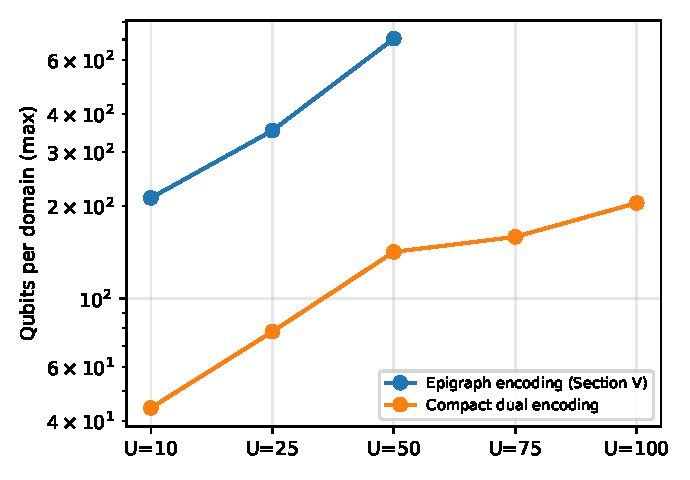
\includegraphics[width=0.85\columnwidth]{figures/qubits_compact_vs_epigraph.pdf}
\caption{Qubits per domain of the compact formulation~\eqref{eq:Nk_compact} and of the direct epigraph encoding of
$\mathscr{P}_3$ (one epigraph register and one slack register per scenario) for the instances of Section~VI.}
\label{fig:qubits}
\end{figure}

%-----------------------------------------------------------------------
\subsection{Ising Mapping and XY-Mixer QAOA}
\label{sec:qaoa}
%-----------------------------------------------------------------------

The QUBO is mapped to an Ising Hamiltonian through the substitution $y_a=(1-\sigma^{z}_{a})/2$, where $a$ indexes the
$\hat N_k$ qubits of the domain and $\sigma^z_a$ is the Pauli-$Z$ operator on qubit $a$. Discarding additive constants,
\begin{align}
    H_{C}^{(k)}&=\sum_{a} h_{a}\,\sigma^{z}_{a}+\sum_{a<a'}J_{aa'}\,\sigma^{z}_{a}\sigma^{z}_{a'},
    \nonumber\\
    h_{a}&=-\frac{1}{2}\sum_{a'}Q^{(k)}_{aa'},\qquad J_{aa'}=\frac{1}{2}Q^{(k)}_{aa'},
    \label{eq:Hc}
\end{align}
where the sums over $a'$ run over the symmetric matrix $\mathbf{Q}^{(k)}$. Couplings $J_{aa'}$ arise only between
candidates that use the same node, and between those candidates and the node's slack bits, so the cost layer is
sparse: the candidates of one UE are not coupled to each other, and candidates at different nodes are not coupled at
all.

For the mixer we do not use the transverse field $\sum_a\sigma^x_a$, which would leave the one-hot subspace and
force D1 back into the cost as a penalty. Instead, on each UE group we apply a ring of XY interactions and keep the
transverse field only on the slack bits~\cite{Hadfield2019}:
\begin{equation}
    H_{M}^{(k)}=\sum_{i\in\mathscr{U}_k}\ \sum_{(a,a')\in\mathrm{ring}(\mathscr{C}_i)}
    \tfrac{1}{2}\bigl(\sigma^x_a\sigma^x_{a'}+\sigma^y_a\sigma^y_{a'}\bigr)
    +\sum_{a\in\mathrm{slack}}\sigma^x_a ,
    \label{eq:HM_xy}
\end{equation}
where $\mathrm{ring}(\cdot)$ denotes adjacent pairs in a cyclic ordering of the group. Each XY term conserves the
Hamming weight of its group, so every Trotter factor of $e^{-\mathrm{i}\theta H_M^{(k)}}$ does as well, and a state
initialized in the one-hot subspace stays in it exactly; the only way a measured sample can violate D1 is through
hardware noise, which the decoder detects. Each group is initialized either in its $W$ state, the uniform
superposition of its one-hot basis states, prepared with a linear-depth ladder of controlled rotations, or in the
basis state of the greedy assignment of Section~V-E, which we call the warm start. The depth-$p$ state is
\begin{equation}
    |\boldsymbol{\gamma},\boldsymbol{\theta}\rangle
    =\prod_{l=1}^{p}e^{-\mathrm{i}\theta_{l}H_{M}^{(k)}}e^{-\mathrm{i}\gamma_{l}H_{C}^{(k)}}\,|\psi_0\rangle,
    \label{eq:qaoa_state}
\end{equation}
and the angles $(\boldsymbol{\gamma},\boldsymbol{\theta})$ are optimized by a derivative-free classical optimizer on
the sampled energy $\langle H_C^{(k)}\rangle$. The sampled bitstrings are decoded classically; samples that are not
one-hot or exceed a capacity are discarded, and the feasible sample with the smallest value of~\eqref{eq:Fk_compact}
is returned as $\hat{\mathbf{x}}_k$. When $\hat N_k$ exceeds the capacity of the available device or simulator, the
inner step is performed by a one-hot-preserving simulated annealer on the same QUBO, which moves one UE's selection
at a time; Section~VI reports which solver produced each result.

%-----------------------------------------------------------------------
\subsection{Distributed Coordination}
\label{sec:admm}
%-----------------------------------------------------------------------

The domains are coupled through the satellites they share. For a shared satellite $s_j$, let
$\mathscr{K}_j\subseteq\mathscr{K}$ be the $K_j$ domains that see it. The coordinator assigns each
$k\in\mathscr{K}_j$ a bandwidth target $z_{jk}$ and keeps a scaled dual variable $u_{jk}$; the local QUBOs carry the
coordination term of~\eqref{eq:Fk_compact}. After the domains return $\hat{\mathbf{x}}_k^{(r+1)}$ in round $r$, the
coordinator sets $\tilde{a}_{jk}=b_j(\hat{\mathbf{x}}_{k}^{(r+1)})+u_{jk}^{(r)}$ and applies the sharing-form ADMM
updates~\cite{Boyd2011}
\begin{align}
    z_{jk}^{(r+1)}&=\tilde{a}_{jk}-\frac{1}{K_j}\max\Bigl\{0,\;\sum_{k'\in\mathscr{K}_j}\tilde{a}_{jk'}-B^{s}_{j}\Bigr\},
    \label{eq:z_update}\\
    u_{jk}^{(r+1)}&=u_{jk}^{(r)}+b_j\bigl(\hat{\mathbf{x}}_{k}^{(r+1)}\bigr)-z_{jk}^{(r+1)},
    \label{eq:u_update}
\end{align}
which lower every target at an overloaded satellite by an equal share of the excess and accumulate the remaining
violation in the duals. The round ends when the primal residual $\bigl(\sum_{j,k}(b_j(\hat{\mathbf{x}}_k^{(r+1)})
-z_{jk}^{(r+1)})^2\bigr)^{1/2}$ and the dual residual $\varrho\bigl(\sum_{j,k}(z_{jk}^{(r+1)}-z_{jk}^{(r)})^2\bigr)^{1/2}$
fall below a tolerance or after $R_{\max}$ rounds; $\varrho$ is adapted by residual balancing.

Two details decide whether this loop produces good schedules, and both were learned from failures. First, the targets
are initialized from an uncoupled round ($\varrho=0$), projected onto capacity, and not from the equal share
$B_j/K_j$. With equal-share targets and the two-sided quadratic coordination term, every domain is pulled toward using
exactly its share of every shared satellite whether or not it needs it, and the loop declares convergence after two
rounds at a schedule that we measured to be 60 to 560\% above the optimum at 50 to 100 UEs. Second, $\varrho$ is scaled
to the mean per-UE spread of the weighted costs $a_v$, so that one bandwidth unit of deviation from the target costs
about one typical per-UE cost difference; a penalty two orders of magnitude larger than the cost differences, which
is what a generic choice produced, makes the coordination term the only thing the inner solver sees. If no
capacity-feasible network schedule has been found when the loop stops, a greedy repair moves UEs from overloaded
satellites to the candidate with the smallest increase in worst-case cost at a node with spare capacity. The
complete procedure is given in Algorithm~\ref{alg:SENTINEL}.

\begin{algorithm}[!t]
\caption{SENTINEL: Distributed Robust Orchestration for VANGUARD}
\label{alg:SENTINEL}
\SetKwInOut{Input}{Input}
\SetKwInOut{Output}{Output}
\Input{$\mathscr{U},\mathscr{S},\mathscr{B}$, $\{P_i\}$, capacities, budgets, levels, $\Theta$, $\mathscr{L}$,
$\kappa$, $T$, $\sigma$, $p$, $R_{\max}$, $\epsilon_{\mathrm{tol}}$.}
\Output{$\mathbf{x}^{\star}$ decoded into $\rho_i$, $\alpha_{ij}$, $\omega_{in}$, $\beta^{us}_{ij}$,
$\beta^{ub}_{in}$; certificate $\eta^{\star}$; worst scenario $\ell^{\star}$.}
\nl Partition the network into $K$ domains; identify shared SATs.\\
\nl Tabulate $\Psi_i(\cdot)$ by~\eqref{eq:psi_def}, the costs $\psi^{(\ell)}_{imqh}$ by~\eqref{eq:psi_imqh}, the
    admissible sets $\mathscr{A}_i$ and the pruned candidates $\mathscr{C}_i$.\\
\nl $\mathbf{w}^{(1)}\leftarrow$ uniform; $\eta^{\star}\leftarrow+\infty$.\\
\nl \For{$t=1,\ldots,T$}{
\nl Warm start: solve each domain with $\varrho=0$; set $z_{jk}^{(0)}$ to the projected loads, $u_{jk}^{(0)}\leftarrow 0$;
    scale $\varrho$ to the cost spread.\\
\nl \For{$r=0,\ldots,R_{\max}-1$}{
\nl \For{each domain $k$ \emph{in parallel}}{
\nl Build $F_k$ by~\eqref{eq:Fk_compact} with $\mathbf{w}^{(t)}$, $\mathbf{z}_k^{(r)}$, $\mathbf{u}_k^{(r)}$; map to
    $H_C^{(k)}$ by~\eqref{eq:Hc}.\\
\nl \lIf{$\hat N_k$ fits the sampler}{run XY-mixer QAOA~\eqref{eq:qaoa_state}, decode, keep the best feasible
    sample as $\hat{\mathbf{x}}_k^{(r+1)}$}
\nl \lElse{obtain $\hat{\mathbf{x}}_k^{(r+1)}$ by one-hot-preserving annealing of $F_k$}
}
\nl Update $z_{jk}^{(r+1)}$, $u_{jk}^{(r+1)}$ by~\eqref{eq:z_update}--\eqref{eq:u_update}; adapt $\varrho$.\\
\nl \If{$\hat{\mathbf{x}}^{(r+1)}$ satisfies D1--D3 and $\max_\ell c^{(\ell)}(\hat{\mathbf{x}}^{(r+1)})<\eta^{\star}$}{
    $\mathbf{x}^{\star}\leftarrow\hat{\mathbf{x}}^{(r+1)}$; $\eta^{\star}\leftarrow\max_\ell c^{(\ell)}(\mathbf{x}^{\star})$.}
\nl \lIf{residuals $\leq\epsilon_{\mathrm{tol}}$}{\textbf{break}}
}
\nl \lIf{no feasible schedule in this iteration}{apply greedy repair and evaluate~\eqref{eq:cert}}
\nl $\mathbf{x}^{(t)}\leftarrow$ best schedule of this iteration; update $\mathbf{w}^{(t+1)}$ by~\eqref{eq:eg}.\\
}
\nl Decode $\mathbf{x}^{\star}$; $\ell^{\star}\leftarrow\arg\max_{\ell}c^{(\ell)}(\mathbf{x}^{\star})$.\\
\end{algorithm}

\textbf{Convergence and certification.} For convex local problems the sharing form of ADMM converges~\cite{Boyd2011};
here the local problems are binary, so the loop is a heuristic and neither it nor the outer weight iteration is
guaranteed to reach the saddle point of~\eqref{eq:dual_max}. SENTINEL does not rely on either for correctness. The
incumbent is replaced only by network schedules that satisfy D1 to D3, and its worst-case AoII~\eqref{eq:cert} is
computed exactly, so the number of iterations affects the quality of the returned schedule but never the validity of
its certificate.

%-----------------------------------------------------------------------
\subsection{Resource Scaling and Complexity}
\label{sec:complexity}
%-----------------------------------------------------------------------

\textbf{Qubits and gates.} By~\eqref{eq:Nk_compact} the qubit count of a domain grows with $\kappa|\mathscr{U}_k|$ and
the slack registers, and does not depend on $L$. Because the cost Hamiltonian couples only candidates that share a
node, the cost layer of domain $k$ needs at most $\sum_{m}\binom{n_{m}+W_m}{2}$ two-qubit $ZZ$ rotations, where
$n_m$ is the number of candidates at node $m$ in the domain and $W_m=0$ for shared satellites; the XY mixer adds
$|\mathscr{C}_i|$ two-qubit rotations per UE group and layer, and the $W$-state preparation $|\mathscr{C}_i|-1$. On a
heavy-hex processor, routing a domain of 18 to 24 qubits yielded 58 to 305 two-qubit gates after transpilation at depth
1, and 606 gates for a 38-qubit domain (Section~VI-E). The direct epigraph encoding, whose scenario penalties couple
every pair of local variables, needs $\hat N_k(\hat N_k-1)/2$ rotations per layer with $\hat N_k$ three to five times
larger.

\textbf{Time.} The offline tabulation of $\Psi_i$ costs $\mathcal{O}(Y^{\max}|\mathcal{X}_i|^3+|\mathcal{X}_i|
(Y^{\max})^2)$ per UE and the coefficients $\psi^{(\ell)}_{imqh}$ cost $\mathcal{O}(L\sum_i|\mathscr{A}_i|)$ lookups,
once per set of sources and scenarios. Assembling and mapping $F_k$ costs $\mathcal{O}(\hat N_k^2)$. If the angle
optimizer runs $I_{\mathrm{QAOA}}$ iterations with $N_{\mathrm{shot}}$ shots each, the quantum work of domain $k$ per
round is $\mathcal{O}(I_{\mathrm{QAOA}}\,p\,N_{\mathrm{shot}}\,G_k)$ with $G_k$ the gate count above, the ADMM updates
cost $\mathcal{O}(\sum_j K_j)$ per round, and the certificate costs $\mathcal{O}(L|\mathscr{U}|)$. With the domains
run in parallel, the wall-clock cost of a solve is
\begin{equation}
    C_{\mathrm{SENTINEL}}=\mathcal{O}\!\Bigl(T\,R_{\max}\bigl(I_{\mathrm{QAOA}}\,p\,N_{\mathrm{shot}}\max_k G_k
    +L|\mathscr{U}|\bigr)\Bigr).
    \label{eq:complexity}
\end{equation}
In the evaluation, a solve of a 20-UE network with $T=6$ and $R_{\max}=20$ took 1 to 7 seconds on the classical
annealer and the orchestration loop used 34 to 223 seconds of solver time per 10-minute run, which is reported rather
than assumed in the AoII figures through the overhead $\epsilon_i$ of Section~III-G. Exhaustive search over
$\mathscr{P}_2$ costs $\mathcal{O}(L|\mathscr{U}|\prod_i|\mathscr{A}_i|)$, and branch-and-cut on $\mathscr{P}_3$ has
the same worst case although it is fast on our instances; a centralized QAOA would need $\sum_k\hat N_k$ qubits on one
device. The advantage of the decomposition is therefore the qubit count per device, not asymptotic time, and
Section~VI reports at which size the inner sampler and the coordination each stop being exact.

% Section VI: Performance Evaluation
%=======================================================================
\section{Performance Evaluation}
\label{sec:performance}
%=======================================================================

We evaluate SENTINEL with the simulator released with this paper\footnote{\url{https://github.com/tanzimulalam/Quantum_SAGIN_AoII_Updated_Simulation}, tag \texttt{v2.2-manuscript}; the script \texttt{scripts/reproduce\_all.sh} regenerates every table and figure.}
under the parameters of Table~\ref{tab:simulation_parameters}, which are the values used for every figure. Each
configuration runs for 60{,}000 slots of 10~ms, ten minutes of network time, on 30 independent seeds; the policies of
one seed share its topology, source trajectories, fading, and disruption realization, so all comparisons are paired.
We report medians with interquartile ranges, because a few seeds contain long non-line-of-sight passes that dominate
means; means with 95\% confidence intervals, the raw per-seed results, and the paired test tables are in the
repository.

\begin{table}[t]
\centering
\caption{Simulation Parameters (values used for all figures)}
\label{tab:simulation_parameters}
\scriptsize
\renewcommand{\arraystretch}{1.12}
\begin{tabular}{p{0.46\columnwidth} p{0.46\columnwidth}}
\hline
\textbf{Parameter} & \textbf{Value} \\
\hline
\multicolumn{2}{l}{\emph{Network}} \\
Number of UEs & $\{5,10,15,20\}$; up to 100 in Sec.~VI-D \\
BSs / satellite serving slots & 2 / 2 (topology study: 0 to 3 each) \\
Area; BS height; UE height & $20\times20$~km$^2$; 25~m; 1.5~m \\
Satellite passes & Starlink TLE snapshot, SGP4, MTSU site (35.85$^\circ$N, 86.39$^\circ$W); min.\ elevation $25^\circ$ \\
Domains $K$ & 2 (one BS each; satellites shared) \\
\hline
\multicolumn{2}{l}{\emph{Channel and resources}} \\
UE transmit power & 23~dBm \\
UE--BS link & 3.5~GHz, 20~MHz, $-147.55+20\log_{10}f+26\log_{10}d+6$~dB, BS gain 15~dBi, NF 7~dB \\
UE--SAT link & 12~GHz, 50~MHz, free space $+1$~dB, gains 30 $+$ 30~dBi, NF 9~dB \\
NTN large-scale model & TR~38.811 suburban (LOS prob., clutter, shadow fading per pass); atm.\ $0.5$~dB$/\sin V$ \\
Bandwidth levels $\bar\beta^q_m$ ($Q_m=3$) & $\{2.5,5,10\}$~MHz, $\Delta_\beta=2.5$~MHz \\
Spectral-efficiency cap & 6 (BS), 4 (SAT) bit/s/Hz \\
\hline
\multicolumn{2}{l}{\emph{Source and AoII}} \\
Source states; transition matrix & 4; birth--death, self-transition $\mathcal{U}[0.90,0.99]$ per UE \\
Distortion; AoII budget $\Delta^{II,\max}_i$ & $|x-\hat x|$; 10 \\
Update periods ($H_i=4$); slot; packet & $\{5,10,20,50\}$ slots; 10~ms; 20~kbit \\
\hline
\multicolumn{2}{l}{\emph{Disruption}} \\
Scenario set ($L=5$) & nominal; deep shadowing 12~dB for 30 slots; handover of each SAT (20 slots); joint loss (30 slots) \\
Realized process (per 1~s interval) & TR~38.811 state per pass; shadowing event per UE--SAT link w.p.\ 0.07; handover failure per SAT w.p.\ 0.03; natural handovers \\
Link-failure handling (all policies) & node blocked after 60 failed slots, for 6~s or until its next handover; SENTINEL re-solves \\
\hline
\multicolumn{2}{l}{\emph{Solver}} \\
Formulation & compact dual, $\kappa=4$, $T=6$ outer iterations, $\sigma=2$ \\
Local solver & XY-QAOA, depth 1, 512 shots, COBYLA 40 it.\ ($\le 26$ qubits); one-hot annealing otherwise \\
ADMM $\varrho_0$, tolerance, rounds & scaled to cost spread, $10^{-2}$, 20 \\
Re-solve & on visibility change, on link failure, at least every 30~s \\
Quantum backend & Qiskit Aer~\cite{Qiskit2024}; FakeTorino / FakeFez; \texttt{ibm\_kingston}, \texttt{ibm\_fez} \\
\hline
\end{tabular}
\end{table}

\textbf{Baselines.} \emph{Random} transmits with probability 0.1 per slot over a uniformly chosen visible node with
equal bandwidth sharing. \emph{AoII threshold} is a state-aware policy that transmits whenever its AoII is positive,
at most once per 5 slots, on the node with the best nominal rate. \emph{Whittle index} is the restless-bandit
scheduler of the AoII literature~\cite{Whittle1988, Kadota2018}: the index of each UE's (source state, estimate, age)
arm is computed numerically per source by relative value iteration on a grid of transmission prices, and every slot
the mismatched UEs are ranked by index and admitted at their best node while the node's shared bandwidth still
delivers every admitted packet; it has the threshold policy's observations and rate cap. \emph{PPO} is an actor-critic
agent~\cite{Schulman2017} that selects, once per orchestration interval, a serving node and an update-period level for
every UE, with invisible or failed nodes masked and equal bandwidth sharing, rewarded with the negative mean AoII of
the interval; it is trained for 5000 episodes per network size on 30 seeds disjoint from the evaluation seeds and
evaluated deterministically on the same episodes as every other policy. \emph{Nominal SENTINEL} runs Algorithm~1
with the nominal scenario alone ($L=1$). \emph{SENTINEL} is the robust schedule with the five-scenario set. \emph{SENTINEL
+ trigger} uses SENTINEL's association and bandwidth with transmissions triggered by the observed mismatch,
rate-capped at the chosen period. Every policy receives the same acknowledgement feedback and applies the same
link-failure rule of Section~III-F. The exact reference for Section~VI-D is the integer linear program
$\mathscr{P}_3$ solved with HiGHS~\cite{HiGHS2018}.

%-----------------------------------------------------------------------
\subsection{AoII Versus Network Size}
\label{sec:ue_sweep}
%-----------------------------------------------------------------------

\begin{figure}[!t]
\centering
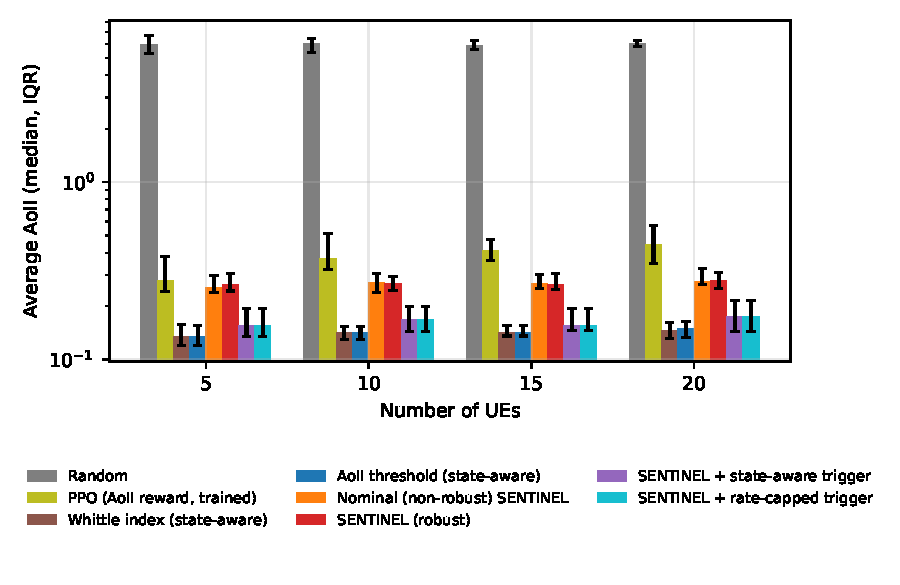
\includegraphics[width=0.86\columnwidth]{figures/ue_sweep_average_aoii_median_disruption_on.pdf}
\caption{Median average AoII (bars) and interquartile range (whiskers) over 30 seeds versus the number of UEs, with
Starlink passes, the TR~38.811 channel, and the stochastic disruption process active.}
\label{fig:ue_sweep}
\end{figure}

Fig.~\ref{fig:ue_sweep} and Table~\ref{tab:tle} give the median average AoII from 5 to 20 UEs. Three groups are
visible. The state-aware per-slot policies, AoII threshold and Whittle index, are lowest at 0.13 to 0.15 and coincide
(Section~VI-C). The SENTINEL schedules, robust and nominal, sit at 0.25 to 0.28 and do not grow with the number of
UEs, because bandwidth levels are dedicated and a re-solve redistributes load as satellites come and go. SENTINEL with
the state-aware trigger lies between the two at 0.155 to 0.175: it keeps the robust association and bandwidth,
transmits only when the estimate is wrong, and thereby raises the informative-update ratio from 0.23 to 0.96 while
retaining the certificate. Random scheduling is at 6; the trained PPO agent matches the nominal schedule at 5 UEs
(0.280 against 0.253), degrades to 0.446 at 20 UEs as its action space grows, routes all traffic to satellites, and,
like SENTINEL, samples without observing the source. Delivery ratios are 0.92 to 0.94 for every policy except random;
the per-slot policies deliver with 2.8 to 3.0~ms of end-to-end latency against 4.7 to 5.8~ms for the SENTINEL
schedules, whose dedicated levels are smaller than an equal share of an otherwise idle node. The satellite tier
carries 73 to 79\% of robust SENTINEL's deliveries and 97 to 98\% of the threshold policy's. Peak AoII is 100 to 400
for every policy and is set by handover interruptions and non-line-of-sight passes rather than by the scheduler. A
20-UE solve used 20 to 58 qubits per domain and the orchestration loop 34 to 223~s of solver time per run.

\begin{table}[!t]
\centering
\caption{Median Average AoII with Starlink Passes and the TR~38.811 Channel (30 seeds, disruption on)}
\label{tab:tle}
\footnotesize
\resizebox{\columnwidth}{!}{%
\begin{tabular}{|c|c|c|c|c|c|c|c|}
\hline
\textbf{UEs} & \textbf{Random} & \textbf{PPO} & \textbf{Whittle} & \textbf{AoII thr.} & \textbf{Nominal} & \textbf{SENTINEL} & \textbf{+ trigger} \\
\hline
5  & 5.94 & 0.280 & 0.134 & 0.134 & 0.253 & 0.265 & 0.155 \\
10 & 6.06 & 0.372 & 0.141 & 0.142 & 0.270 & 0.269 & 0.168 \\
15 & 5.87 & 0.413 & 0.142 & 0.142 & 0.269 & 0.264 & 0.155 \\
20 & 6.05 & 0.446 & 0.146 & 0.149 & 0.276 & 0.278 & 0.175 \\
\hline
\end{tabular}%
}
\end{table}

%-----------------------------------------------------------------------
\subsection{The Certificate and the Value of Robustness}
\label{sec:certificate}
%-----------------------------------------------------------------------

\begin{figure}[!t]
\centering
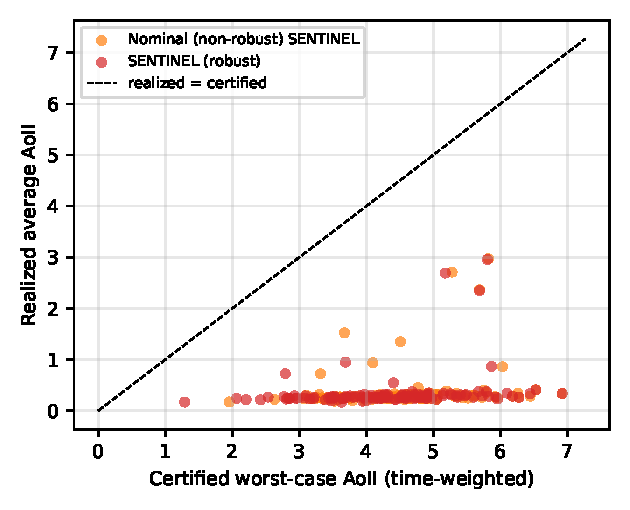
\includegraphics[width=0.78\columnwidth]{figures/certificate_vs_realized.pdf}
\caption{Certified worst-case AoII of each orchestration run against its realized average AoII, robust and nominal
SENTINEL, all sizes and seeds of Fig.~\ref{fig:ue_sweep}. Points below the diagonal stayed within the certificate.}
\label{fig:certificate}
\end{figure}

Fig.~\ref{fig:certificate} plots the certified worst case of every run against the AoII it realized. The realized
average stayed within the certificate in 98.7\% of orchestration epochs for the robust schedule and 98.5\% for the
nominal one; the violations are passes that enter the non-line-of-sight state, whose 17 to 25~dB clutter loss exceeds
the 12~dB deep-shadowing scenario. With a synthetic pass model that produces coverage gaps longer than any scenario
window the figure was 98.0\%, and every violation there was such a gap. The certificate is therefore valid against the
scenario set it was computed from, and the paper states its scope that way.

What the scenario set buys is visible in the certificate, not in the realized AoII. Across the 30 paired seeds the
robust schedule's certified worst case is 2 to 7\% below the nominal schedule's (paired-median ratio 0.93 at 5 UEs to
0.98 at 20 UEs), lower in 67 to 100\% of seeds, with Wilcoxon signed-rank $p\le 9\times10^{-5}$ at every size after
Holm correction. The realized AoII of the two is statistically indistinguishable at every size ($p\ge0.08$), although
the robust mean at 20 UEs is lower, 0.39 against 0.46, because the robust schedule keeps 21 to 27\% of deliveries on
base stations. The gap between SENTINEL with the trigger and the threshold policy, 0.02 to 0.03 in AoII, is small but
significant at every size ($p\le0.013$), and PPO is significantly behind SENTINEL from 10 UEs on.

\begin{figure}[!t]
\centering
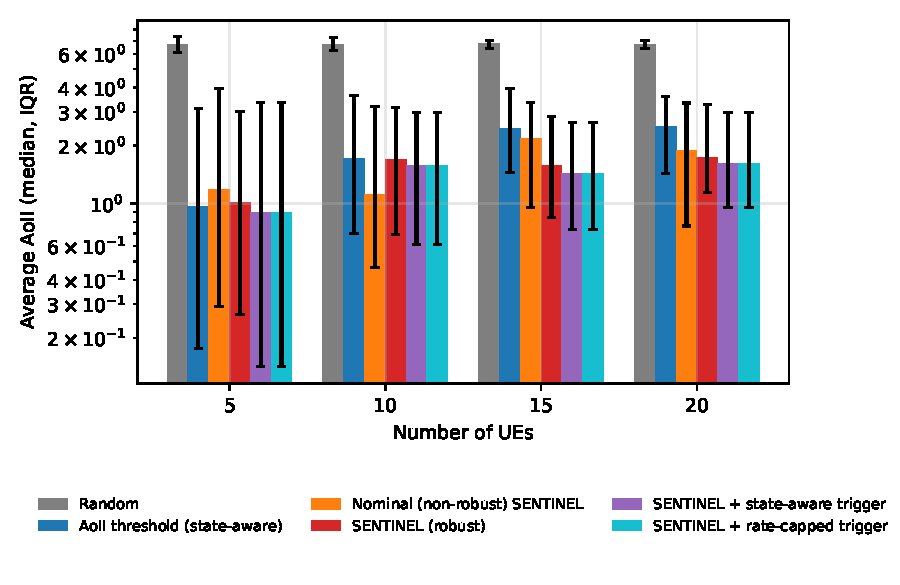
\includegraphics[width=0.86\columnwidth]{figures/noack_ue_sweep_average_aoii_median.pdf}
\caption{Median average AoII (60 seeds) with acknowledgement feedback and link-failure handling disabled for every
policy.}
\label{fig:noack}
\end{figure}

\textbf{Without failure feedback.} Whether the network can react to a dead link matters more than any scheduling
choice. Fig.~\ref{fig:noack} repeats the sweep with the link-failure rule disabled for every policy, on 60 seeds
because the distributions become heavy-tailed. Median AoII rises by an order of magnitude for all policies, the
certificate holds in 87 to 92\% of epochs, and the threshold policy, which concentrates 98\% of its traffic on the best
nominal satellite, ties the SENTINEL schedules at 5 and 10 UEs and falls 25 to 30\% behind SENTINEL with the trigger
at 15 and 20 UEs (Hodges-Lehmann differences $-0.77$ and $-0.71$, Holm-corrected $p=0.023$ and $0.029$), while the
SENTINEL schedules keep 18 to 27\% of deliveries on base stations. Robust and nominal SENTINEL remain
indistinguishable in realized AoII here as well ($p\ge0.41$). The measurable product of the robust scenario set is
thus its lower certificate, obtained in both regimes, and the measurable value of a scheduled base-station share
appears when feedback is absent.

\textbf{Scenario-set size.} To see which scenarios matter, the list was extended by a mild 6~dB shadowing scenario and
truncated to $L=1,\ldots,6$ at 10 UEs. Realized AoII is flat in $L$ (0.265 to 0.278); the certificate and the
base-station hedge move only once the handover of the second shared satellite enters the set, the certified worst
case falling from 4.57 to 4.28 and the satellite share from 0.79 to 0.74 between $L=4$ and $L=5$. The mild scenario
never binds: removing it from the full set leaves the certified worst case of every schedule unchanged on all 30 seeds
at every size, with realized-AoII differences below $10^{-3}$, which is why the paper's scenario set has five members.

%-----------------------------------------------------------------------
\subsection{Topology, the Whittle Index, and Capacity}
\label{sec:topology}
%-----------------------------------------------------------------------

\begin{figure}[!t]
\centering
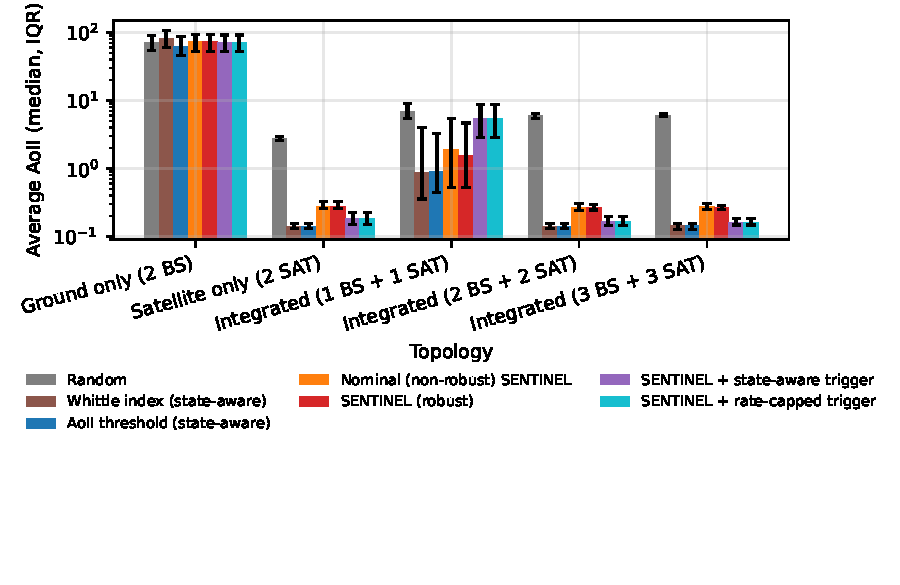
\includegraphics[width=0.86\columnwidth]{figures/topology_average_aoii_median.pdf}
\caption{Median average AoII at 10 UEs for ground-only, satellite-only, and integrated deployments (30 seeds,
disruption on, logarithmic scale).}
\label{fig:topology}
\end{figure}

Fig.~\ref{fig:topology} compares deployments at 10 UEs. Two base stations cover only the UEs within 5 to 7~km of the
$20\times20$~km$^2$ area, so ground-only monitoring fails for every policy (median AoII 63 to 81). Two satellite
serving slots alone bring the per-slot policies to 0.14 and the SENTINEL schedules to 0.18 to 0.28, and the
integrated $2+2$ and $3+3$ deployments are the best for every policy, with SENTINEL routing 26 to 36\% of its
deliveries to base stations. The one deployment in which the SENTINEL schedules are clearly worse than the per-slot
policies is a single base station with a single satellite slot (medians 1.6 to 1.9 against 0.87 to 0.90, and 5.4 for
the triggered hybrid): with one slot, every natural handover is a total outage for every UE on it, and a periodic or
rate-capped schedule loses more during the recovery than a policy that retransmits the moment the link returns. We
report this as a limitation of scheduled transmission at that topology.

\begin{figure}[!t]
\centering
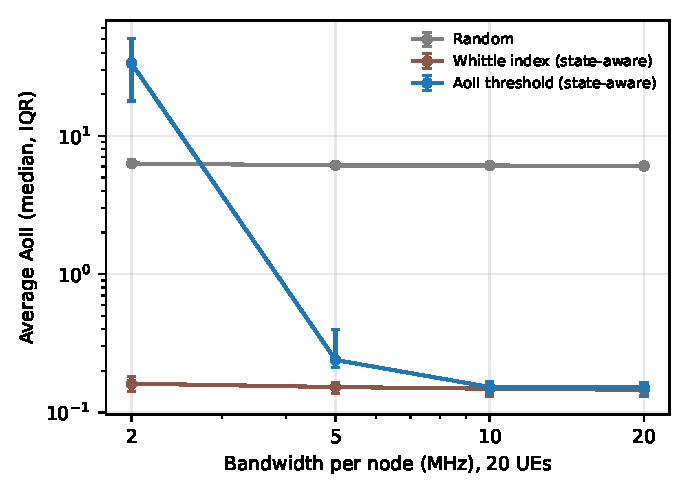
\includegraphics[width=0.8\columnwidth]{figures/capacity_average_aoii.pdf}
\caption{Median average AoII (IQR over 30 seeds) of the per-slot state-aware policies at 20 UEs as the bandwidth per
node is reduced. The Whittle-index scheduler and the AoII-threshold policy coincide while capacity does not bind
and separate below 5~MHz, where uncoordinated threshold transmissions collapse the shared links.}
\label{fig:capacity}
\end{figure}

\textbf{Whittle index and capacity.} At the bandwidths of Table~\ref{tab:simulation_parameters} a node delivers 19 to
40 simultaneous equal sharers within one slot, so capacity never binds and the Whittle scheduler makes the same
decisions as the threshold policy; their AoII is identical to three decimals at every size and in every topology
($p\ge0.18$), and the threshold baseline of this paper is the Whittle-index policy of this regime. Fig.~\ref{fig:capacity}
reduces the bandwidth per node at 20 UEs. At 5~MHz the threshold policy is 57\% worse than the index scheduler
(0.239 against 0.152, $p=4\times10^{-9}$), and at 2~MHz its simultaneous transmissions collapse every shared link
(median AoII 33.5, delivery ratio 0.16) while the capacity-aware index scheduler stays at 0.16. SENTINEL's dedicated
bandwidth levels avoid this regime by construction. The index scheduler's one weakness is the ground-only
deployment, where its admission rule never attempts a node that cannot deliver at the nominal rate and the
threshold policy's blind attempts occasionally succeed on a fading upswing (81 against 63).

%-----------------------------------------------------------------------
\subsection{Validation Against the Exact Minimax Optimum}
\label{sec:exact_validation}
%-----------------------------------------------------------------------

Table~\ref{tab:optimality_gap} reports the mean gap to the exact ILP optimum of $\mathscr{P}_3$ over
capacity-feasible schedules (10 seeds; 5 for the QAOA rows), for the XY-mixer QAOA on the statevector simulator, for
the full distributed pipeline of Algorithm~1 with the compact QUBO and with the epigraph encoding of our earlier
version, and for greedy association refined by local search.
\begin{table}[!t]
\centering
\caption{Mean Optimality Gap (\%) Above the Exact ILP Optimum of $\mathscr{P}_3$}
\label{tab:optimality_gap}
\footnotesize
\resizebox{\columnwidth}{!}{%
\begin{tabular}{|l|c|c|c|c|c|}
\hline
\textbf{Setting} & \textbf{Qubits/domain} & \textbf{XY-QAOA} & \textbf{Compact ADMM} & \textbf{Epigraph ADMM} & \textbf{Greedy+LS} \\
\hline
4--8 UEs, 2+2 & 8--24 & 0.0 (15/15 optimal) & 0.0 & 38--51 & 0.0 \\
10 / 25 UEs, 2+2 & 44 / 78 & -- & 0.0 & 42.7 / 1.8 & 0.0 \\
50 UEs, 4+3 & 142 & -- & 11.5 & 38.8 & 6.0 \\
75 / 100 UEs & 159 / 205 & -- & 49.9 / 60.5 & -- & 14.4 / 11.5 \\
Severity sweep, 20 UEs & 29--66 & -- & 0.0 & 0.2--4.7 & 0.0 \\
$L=1/3/5/6$, 20 UEs & 60--77 & -- & 0.0/3.2/6.9/0.0 & 74/233/9.0/3.8 & 0/0/1.1/0 \\
\hline
\end{tabular}%
}
\end{table}
The XY-mixer QAOA returned the exact optimum on every instance whose domains fit the simulator (8 to 24 qubits),
with 100\% of samples one-hot and capacity-feasible; the epigraph encoding, run with the same classical search, is 38
to 51\% above the optimum on the same instances with 133 to 193 qubits, and a plain simulated annealer on its penalty
landscape found no feasible assignment in 50 solves at 10 UEs. The compact distributed pipeline is exact through 25
UEs and within 12\% at 50; its limit at 75 to 100 UEs is the coordination of five shared satellites among six to eight
domains, which neither more ADMM rounds nor smaller dual steps resolve, and where greedy association with local
search stays within 11 to 14\%. Candidate pruning with $\kappa=4$ never changed the optimum. The exact reference was
solved to proven optimality in under a second on every instance up to 75 UEs and reached its time limit on one in ten
instances at 100 UEs.

%-----------------------------------------------------------------------
\subsection{Quantum Resources and Device Results}
\label{sec:device}
%-----------------------------------------------------------------------

Table~\ref{tab:hardware} lists the transpiled circuits of the hardware-sized domains (depth 1, greedy warm start,
optimization level 3, eight routing trials) and the results of sampling them on the \texttt{ibm\_kingston} and
\texttt{ibm\_fez} processors (Heron r2, 156 qubits, 27 and 28 October 2026; job identifiers in the repository).
Every scenario weight, ADMM target, and QAOA angle was optimized on the simulator; each device job executed only the
final sampling circuit of one or two domains with 4096 shots, and the campaign used 47~s of processor time. The
38-qubit domain exceeds the statevector simulator and received the angles of the largest simulated domain of its run,
relying on the concentration of QAOA parameters across instances~\cite{Brandao2018}. On the FakeTorino and FakeFez
noise models the 18- and 20-qubit domains of the first instance kept 52 and 33\%, and 70 and 48\%, of their shots
feasible, bracketing the device values.
\begin{table}[!t]
\centering
\caption{Transpiled Circuits ($\kappa=4$, depth 1, greedy start) and Device Sampling Results (4096 shots)}
\label{tab:hardware}
\footnotesize
\resizebox{\columnwidth}{!}{%
\begin{tabular}{|l|c|c|c|l|c|c|}
\hline
\textbf{Instance} & \textbf{Dom.} & \textbf{Qubits} & \textbf{2q gates / depth} & \textbf{Device} & \textbf{Feasible shots} & \textbf{Best = opt.} \\
\hline
6 UEs, s1 & 0 & 18 & 139 / 187 & \texttt{ibm\_kingston} & 63.3\% & yes \\
6 UEs, s1 & 1 & 20 & 301 / 428 & \texttt{ibm\_kingston} & 42.7\% & yes \\
6 UEs, s2 & 0 & 18 & 139 / 187 & \texttt{ibm\_kingston} & 60.9\% & yes \\
6 UEs, s2 & 1 & 12 & 58 / 76 & \texttt{ibm\_kingston} & 73.5\% & yes \\
6 UEs, s3 & 0 & 24 & 305 / 387 & \texttt{ibm\_kingston} & 34.8\% & yes \\
6 UEs, s3 & 1 & 14 & 120 / 187 & \texttt{ibm\_kingston} & 69.6\% & yes \\
6 UEs, s5 & 0 & 12 & 58 / 74 & \texttt{ibm\_kingston} & 75.9\% & yes \\
6 UEs, s5 & 1 & 12 & 58 / 74 & \texttt{ibm\_kingston} & 76.4\% & yes \\
6 UEs, s6 & 0 & 8 & 38 / 77 & \texttt{ibm\_fez} & 86.5\% & yes \\
6 UEs, s6 & 1 & 16 & 79 / 77 & \texttt{ibm\_fez} & 61.8\% & yes \\
6 UEs, s7 & 0 & 12 & 58 / 76 & \texttt{ibm\_fez} & 71.9\% & yes \\
6 UEs, s7 & 1 & 18 & 142 / 171 & \texttt{ibm\_fez} & 59.4\% & yes \\
10 UEs, s1 & 0 & 38 & 606 / 626 & \texttt{ibm\_kingston} & 2.6\% & yes \\
\hline
\end{tabular}%
}
\end{table}

Device noise breaks the one-hot structure or the capacity of a part of the shots, which the decoder discards. In all
thirteen domains the best surviving sample equals the noiseless optimum, and every decoded network schedule attains
the exact ILP optimum of its instance. The feasible-shot fraction is the honest measure of the noise: 60 to 86\% at 8
to 18 qubits with up to 139 two-qubit gates, 35 to 43\% at 20 to 24 qubits with about 300 gates, and 2.6\% at 38
qubits with 606 gates. At the 38-qubit scale the device still contains the optimum among 4096 shots, but a few hundred
more two-qubit gates would leave fewer than one feasible shot in a thousand, which places the present limit of the
quantum step at about ten UEs per domain at depth 1. Error suppression does not move it: re-sampling the 24- and
38-qubit domains in one calibration session with dynamical decoupling (XY4)~\cite{Viola1999}, and with dynamical
decoupling plus Pauli twirling~\cite{Wallman2016}, lowered the feasible fraction from the in-session control values of
25.0\% and 2.4\% to 21.1\% and 0.7\%, and to 13.8\% and 0.2\%; these circuits have almost no idle time, so decoupling
pulses add gate error without cancelling idle dephasing, and twirling inserts further single-qubit gates. The best
sample equalled the optimum in every one of those runs. The unmitigated yield of the same circuit also varied by about
ten points between calibration sessions (34.8\% against 25.0\%), so every device comparison here is made within one
session.

On every hardware-sized domain the greedy assignment is already optimal, and the QAOA layers only concentrate a
constrained sampler: from the $W$ state one layer raises the probability of drawing an optimal assignment from the
uniform 0.22 to 0.28 and two layers to 0.42, independently of the shot count above 128, and from the greedy basis
state the optimum is retained with probability 0.99 at depth 1. We therefore claim no quantum advantage. The instances
on which greedy association is suboptimal, 50 UEs and above in Table~\ref{tab:optimality_gap}, need 140 to 200 qubits
per domain, beyond simulation and beyond the gate budget the feasible-shot fractions above allow on current devices;
whether a sampler at that size concentrates on the optimal set is the question this work leaves open.

% Section VII: Conclusion
%=======================================================================
\section{Conclusion}
\label{sec:conclusion}
%=======================================================================

This paper asked how a satellite-ground edge network should schedule status updates when what matters is whether the
edge estimate is correct, and when the satellite links that carry most of the traffic fail for minutes at a time. We
formulated the robust problem VANGUARD, reduced the history-dependent AoII to a tabulated cost per inter-delivery
interval through a renewal-interval decomposition, and solved the resulting minimax assignment with SENTINEL, which
dualizes the minimax into classically updated scenario weights, encodes each domain's linear subproblem as a compact
QUBO whose one-hot structure the XY mixer preserves, coordinates the domains by ADMM, and certifies every schedule by
its exact worst case.

Under Starlink passes and the TR 38.811 channel the certificate held in 98.7\% of epochs, the robust schedule's
certificate was 2 to 7\% below the nominal one while the two were indistinguishable in realized AoII with and without
failure feedback, and SENTINEL with a state-aware trigger came within 10 to 20\% of the best per-slot heuristic, which
coincides with the Whittle-index scheduler at these bandwidths, while beating it by 25 to 30\% at 15 to 20 UEs when
feedback is removed. The compact formulation needs four to five times fewer qubits than a direct epigraph encoding,
is exact through 25 UEs, and is limited at 75 to 100 UEs by the coordination of shared satellites. Thirteen device
domains of 8 to 38 qubits all decoded to the exact optimum, with the fraction of usable shots falling from 86\% to
2.6\% and not improved by error suppression; at these sizes the quantum sampler is correct but not a better optimizer
than greedy association. Three directions follow: a coordinator that negotiates per-UE assignments rather than
aggregate bandwidth, to remove the bottleneck above 50 UEs; a scenario set learned from the pass statistics of the
site, since the handover scenario was the one that mattered; and the open question of whether a constrained quantum
sampler concentrates on the optimal set at the 150-qubit scale where greedy association starts to fail, which will be
answered on hardware rather than in simulation.


%=======================================================================
\bibliographystyle{IEEEtran}
\bibliography{main}

\end{document}
